\chapter{Numerical Results for the Asset Allocation Problem}
\label{ch:numerical_results}

In this chapter we present the numerical results of some of the policy gradient algorithms discussed in Chapter \ref{ch:policy_gradient} for the asset allocation problem. Two different type of markets are analyzed: a market with only one risky asset and a market where multiple risky assets are available, for which finding a trading strategy is more difficult since the state and action spaces are much larger. The learning algorithms are first applied both in their risk-neutral version and risk-sensitive formulation to synthetically generated data, which present profitably tradable features. Once the behavior of these algorithms is validated in this controlled environment, the application on historical price series is considered. 

\section{Synthetic Risky Asset}
\label{sec:synthetic_risky_asset}
To test the different reinforcement learning methods in a controlled environment, we generated log-price series for the risky asset as random walks with autoregressive trend processes. The two-parameter model is thus given by
\begin{equation*}
	\begin{split}
		z_t &= z_{t-1} + \beta_{t-1} + \kappa \epsilon_t\\
		\beta_t &= \alpha \beta_{t-1} + \nu_t\\
	\end{split}
\end{equation*}
We then define the synthetic price series as
\begin{equation*}
	Z_t = \exp\left(\frac{z_t}{\max_t z_t - \min_t z_t}\right)
\end{equation*}
This model is often taken as a benchmark test in the automated trading literature, see for instance \cite{moody1998performance}, because the price series generated in this way present some patterns that can be profitably exploited. Moreover the model is stationary and therefore the policy learned on the training set should generalize well on the test set, also known as backtest in the financial jargon. Thus we would expect our learning algorithms to perform well on this test case. If this wasn't the case, we should go back and improve the learning algorithms.\\
In this setting, we compare three the results of three long-short strategies obtained with ARAC, PGPE and NPGPE in both the risk-neutral and risk-sensitive framework. This means that the agent can either go long on the risky asset (i.e. $a_t^1 = 1$) or short the security (i.e. $a_t^1 = -1$) and invest the proceedings in the risk-less asset. Given the current conditions of the financial markets, we always assume a risk-free rate $X = 0$. Let us describe in more detail the the choice we made for each of the algorithms. 

\subsection{Specifications of the Learning Algorithms}
Let us detail the choice of the parametric policies selected for each learning algorithm.  

\paragraph{ARAC} 
We considered a Boltzmann exploration policy on the two actions $a_t^1 \in \{-1, 1\}$ and a linear critic in which the features coincide with the agent's observation of the system state. This critic is extremely simple and there is surely some work to be done to improve it. 

\paragraph{PGPE}
We considered a binary deterministic controller 
\begin{equation*}
	F_\theta(s) = \sign(\theta \cdot s)
\end{equation*}
where the parameters and the state also include a bias term. The controller parameters are sampled from a multi-variate Gaussian distribution
\begin{equation*}
	\theta \sim \calN(\mu, \diag(\sigma))
\end{equation*}  

\paragraph{NPGPE}
We used the same controller as for PGPE but we assumed that the controller parameters are sampled from a Gaussian distribution parameterized by its mean and Cholesky factor
\begin{equation*}
	\theta \sim \calN(\mu, C^T C)
\end{equation*}  


\subsection{Experimental Setup}   
All the algorithms were tested on the same price series of size $9000$, generated from the process described above using $\alpha = 0.9$ and $\kappa = 3$. The learning process consisted of $1000$ training epochs on the first $7000$ days of the series with a learning rate that decreased at each epoch according to a polynomial schedule. The trained agents were subsequently backtested on the final $2000$ days, during which the agents kept learning online in order to try to adapt to the changing environment. Since the price series is generated using a stationary model, it is not necessary to backtest the algorithm using the rolling-window approach typically employed in practice. The results that we present are the average of $10$ independent experiments that used slightly different random initialization of the policy parameters.   

\subsection{Risk-Neutral Framework}
\subsubsection{Convergence}
\begin{figure}[t!]
	\centering
	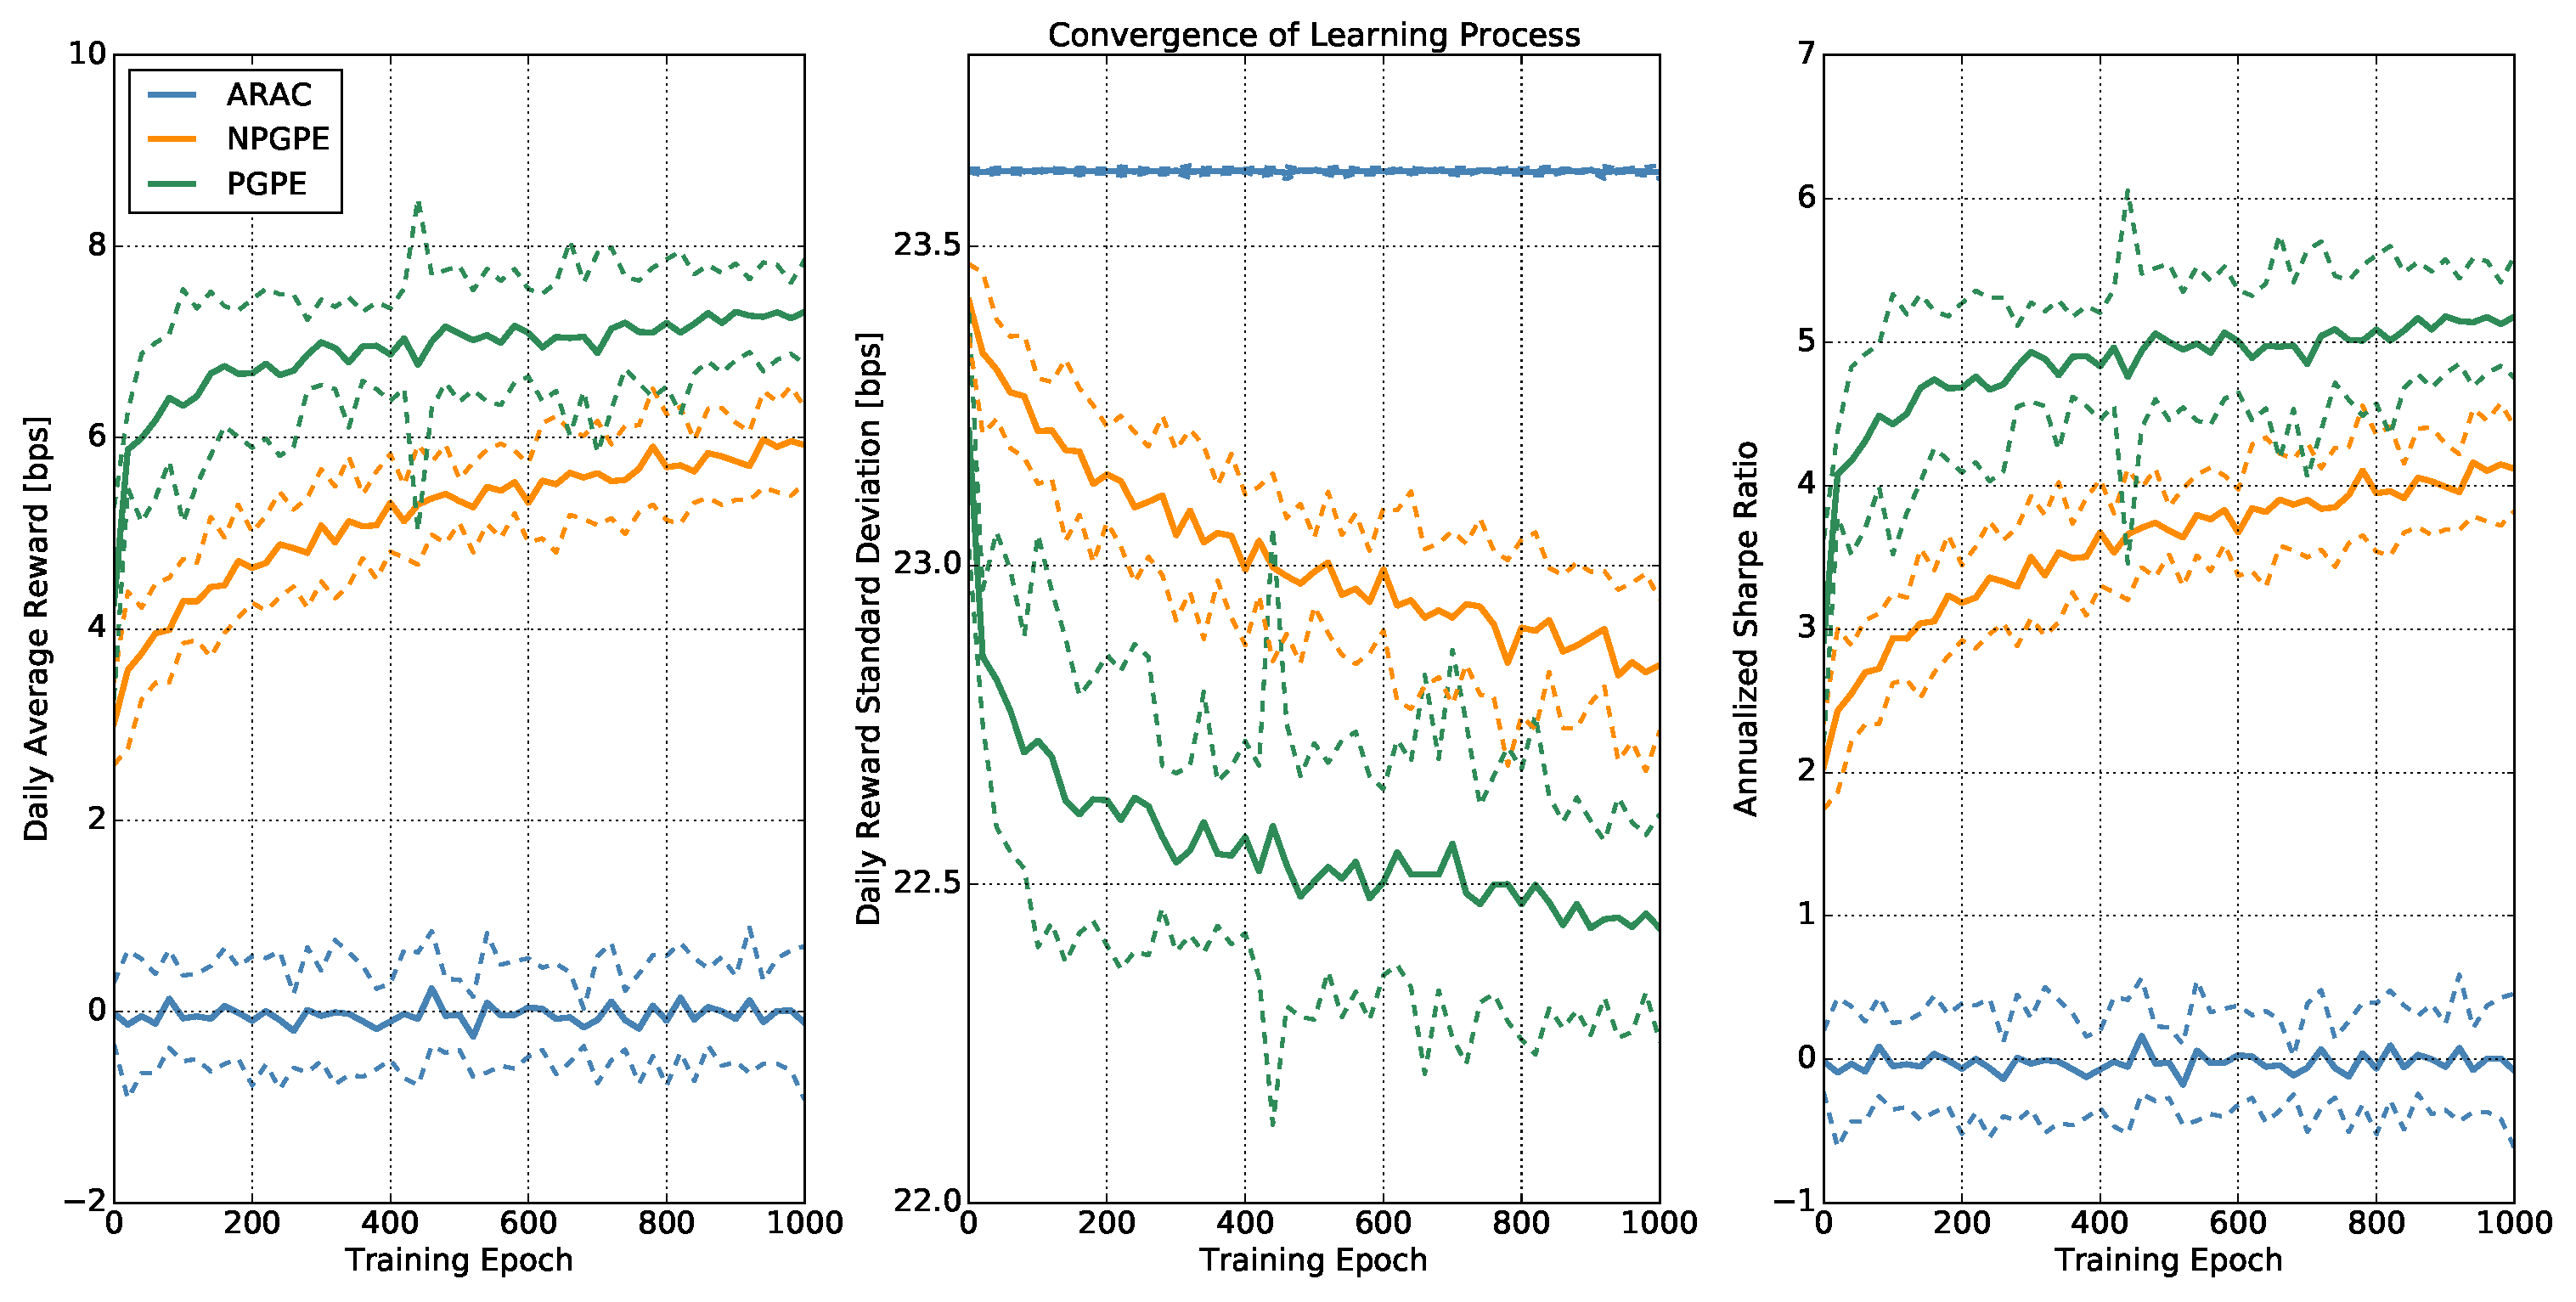
\includegraphics[height=6cm,width=1.0\textwidth]{Images/6_0_single_synthetic_neutral_convergence}
	\caption[Risk-neutral learning process for one synthetic risky asset]{Risk-neutral learning process for the asset allocation problem with one synthetic risky asset.}
	\label{fig:single_synthetic_neutral_convergence}
\end{figure}
Let us first discuss the case with no transaction costs. Figure \ref{fig:single_synthetic_neutral_convergence} shows the learning curves for the three risk-neutral algorithms in terms of average daily reward, which is the quantity being maximized by the algorithms, the daily reward standard deviation and the annualized Sharpe ratio. The first thing we observe is the ARAC algorithm seems not to be improving the trading strategy as the training epochs go by. The average reward obtained is close to zero and will be surely be negative once transaction costs are introduced. On the other hand, NPGPE slowly converges to a profitable strategy which is however suboptimal compared to the one found by PGPE, that is better in all three measures considered. It is interesting to notice that PGPE and NPGPE yield a learning curve for the Sharpe ratio very similar to the one for the average reward. Even if the algorithm is risk-neutral, it manages to improve a risk-senitive measure at the same time of the average reward. This might be simply a peculiarity of the very simple model assumed for the synthetic risky asset. Moreover, since the price process is stationary, the trading strategy learned on the training set perfectly generalizes to the test set. 

\subsubsection{Performances}
Figure \ref{fig:single_synthetic_neutral_performance} compares the backtest performances of the three learned policies and a Buy and Hold strategy, which simply consists in investing all the available capital in the risky asset. Let us repeat that the solid lines are the averages of $10$ independent experiments, which allows us to determine the $95\%$ confidence intervals represented with the dashed lines. We clearly see that NPGPE and PGPE easily beat the market, realizing a total profit of $231.63\%$ and $314.34\%$ respectively against the $7.81\%$ profit of the Buy and Hold strategy over the same period.
\begin{figure}[t]
	\centering
	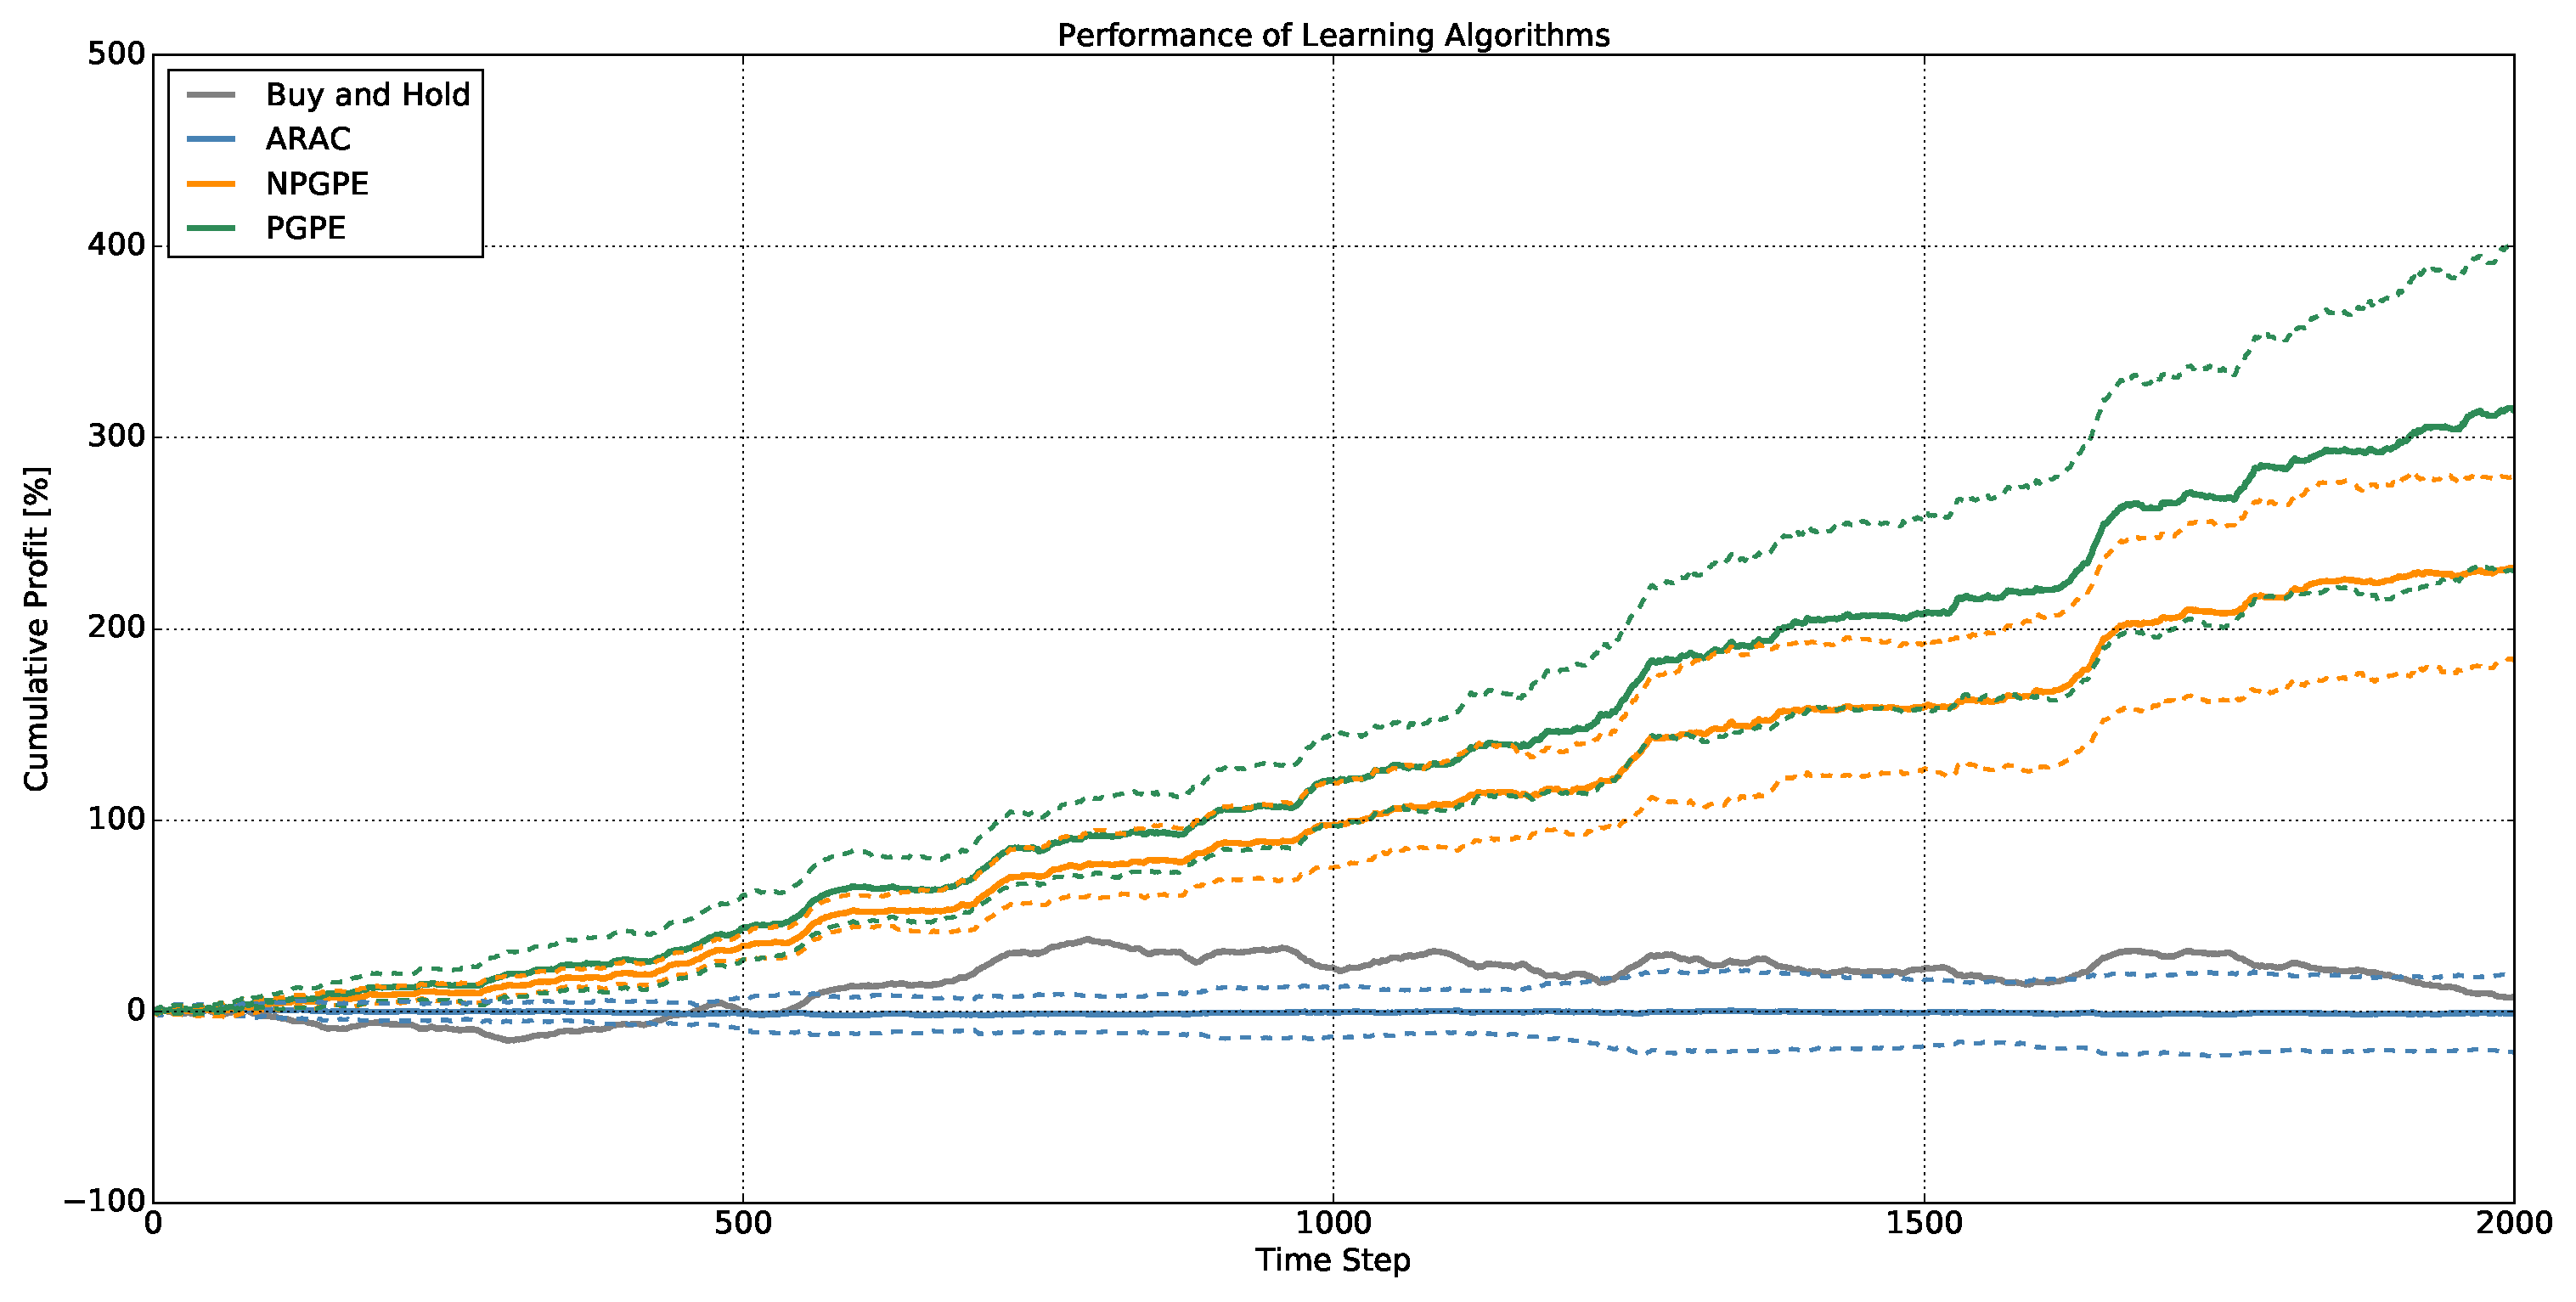
\includegraphics[width=1.0\textwidth]{Images/6_1_single_synthetic_neutral_performance}
	\caption[Backtest performance with one synthetic risky asset]{Backtest performance of trained trading systems for the asset allocation problem with one synthetic risky asset.}
	\label{fig:single_synthetic_neutral_performance}
\end{figure}
Table \ref{tab:single_synthetic_neutral_performance} reports more performance statistics for the trading strategies averaged over the independent experiments. We remark that PGPE and NPGPE beat the simple Buy and Hold strategy with respect to all measures, impressively achieving almost 100\% of profitable years and consecutive 12 months periods. These statistics confirm that ARAC is not able to detect the profitable patterns in the synthetic price series and the learned strategy is close to randomness, with a 50\% probability of reallocation (i.e. a coin flip). On the other hand, PGPE and NPGPE presents much lower reallocation frequencies. This seems promising for dealing with transaction costs, which penalize reallocations and short positions. In the next section we analyze in detail how to behavior of the learned strategies change with the introduction of transaction costs. 


\begin{table}[t!]
\centering
\begin{tabular}{@{}lrrrr@{}}
\toprule
 & \multicolumn{1}{c}{Buy and Hold} & \multicolumn{1}{c}{ARAC} & \multicolumn{1}{c}{NPGPE} & \multicolumn{1}{c}{PGPE} \\ \midrule
Total Return 		& 7.81\% 	& -0.86\% 	& 231.63\% 	& 314.34\% \\
Daily Sharpe 		& 0.27 		& -0.02 	& 4.13 		& 4.95 \\
Monthly Sharpe 		& 0.19 		& -0.07 	& 2.90 		& 3.26 \\
Yearly Sharpe 		& 0.23 		& -0.10 	& 1.55 		& 1.76 \\
Max Drawdown 		& -22.35\% 	& -12.60\% 	& -3.72\% 	& -3.27\% \\
Avg Drawdown 		& -1.75\% 	& -1.81\% 	& -0.49\% 	& -0.43\% \\
Avg Up Month 		& 2.87\% 	& 1.14\% 	& 2.47\% 	& 2.74\% \\
Avg Down Month 		& -2.58\%	& -1.10\% 	& -0.73\% 	& -0.67\% \\
Win Year \% 		& 40.00\% 	& 44.00\% 	& 98.00\% 	& 100.00\% \\
Win 12m \% 			& 56.36\% 	& 48.00\% 	& 100.00\% 	& 100.00\% \\
Reallocation Freq 	& 0.00\% 	& 50.01\% 	& 19.99\% 	& 15.43\% \\
Short Freq 			& 0.00\% 	& 50.13\% 	& 41.59\% 	& 44.25\% \\ \bottomrule
\end{tabular}
\caption[Backtest statistics for risk-neutral learning with one synthetic risky asset]{Backtest statistics of the risk-neutral trading strategies for the asset allocation problem with one synthetic risky asset. \emph{Total Return} is the cumulative return obtained following the strategy. \emph{Daily Sharpe} is the daily Sharpe ratio, annualized. \emph{Monthly Sharpe} is the monthly Sharpe ratio, annualized. \emph{Yearly Sharpe} is the yearly Sharpe ratio. \emph{Max Drawdown} is the maximum drawdown observed, i.e. the maximum loss from a peak to a trough of a portfolio, before a new peak is attained. \emph{Avg Drawdown} is the average drawdown observed, i.e. the average loss from a peak to a through of a portfolio. \emph{Avg Up Month} is the average profit on a positive month. \emph{Avf Down Month} is the average loss on a negative month. \emph{Win Year \%} is the percentage of positive years. \emph{Win 12\%} is the percentage of profitable consecutive 12 months. \emph{Reallocation Freq} is the frequency with which the agent changes its position. \emph{Short Freq} is the frequency with which the agent shorts the risky asset.}
\label{tab:single_synthetic_neutral_performance}
\end{table}

\subsubsection{Impact of Transaction Costs}
In the algorithmic trading literature there are many examples of strategies based on the prediction of future rewards starting from more or less complex indicators. However, as discussed in the previous chapter, the performances of these methods quickly degrade when transaction costs for changing the portfolio composition or for shorting a security are considered. Indeed, these methods simply invest based on the prediction of the future returns, without explicitly taking into account transaction costs. On the other hand, reinforcement learning algorithms should learn to avoid frequent reallocations or shorts thanks to the feedback mechanism between the learning agent and the system, thus generating better trading performances. In this section we analyze how the strategies learned by PGPE and by NPGPE change when gradually increasing the proportional transaction costs and the short-selling fees. Intuitively, we expect a progressive reduction of the frequency of reallocation and of shorting the risky asset.\\
Figure \ref{fig:impact_transaction_costs} shows the impact of proportional transaction costs on the trading strategies learned by PGPE and by NPGPE. 
\begin{figure}[t!]
	\centering
	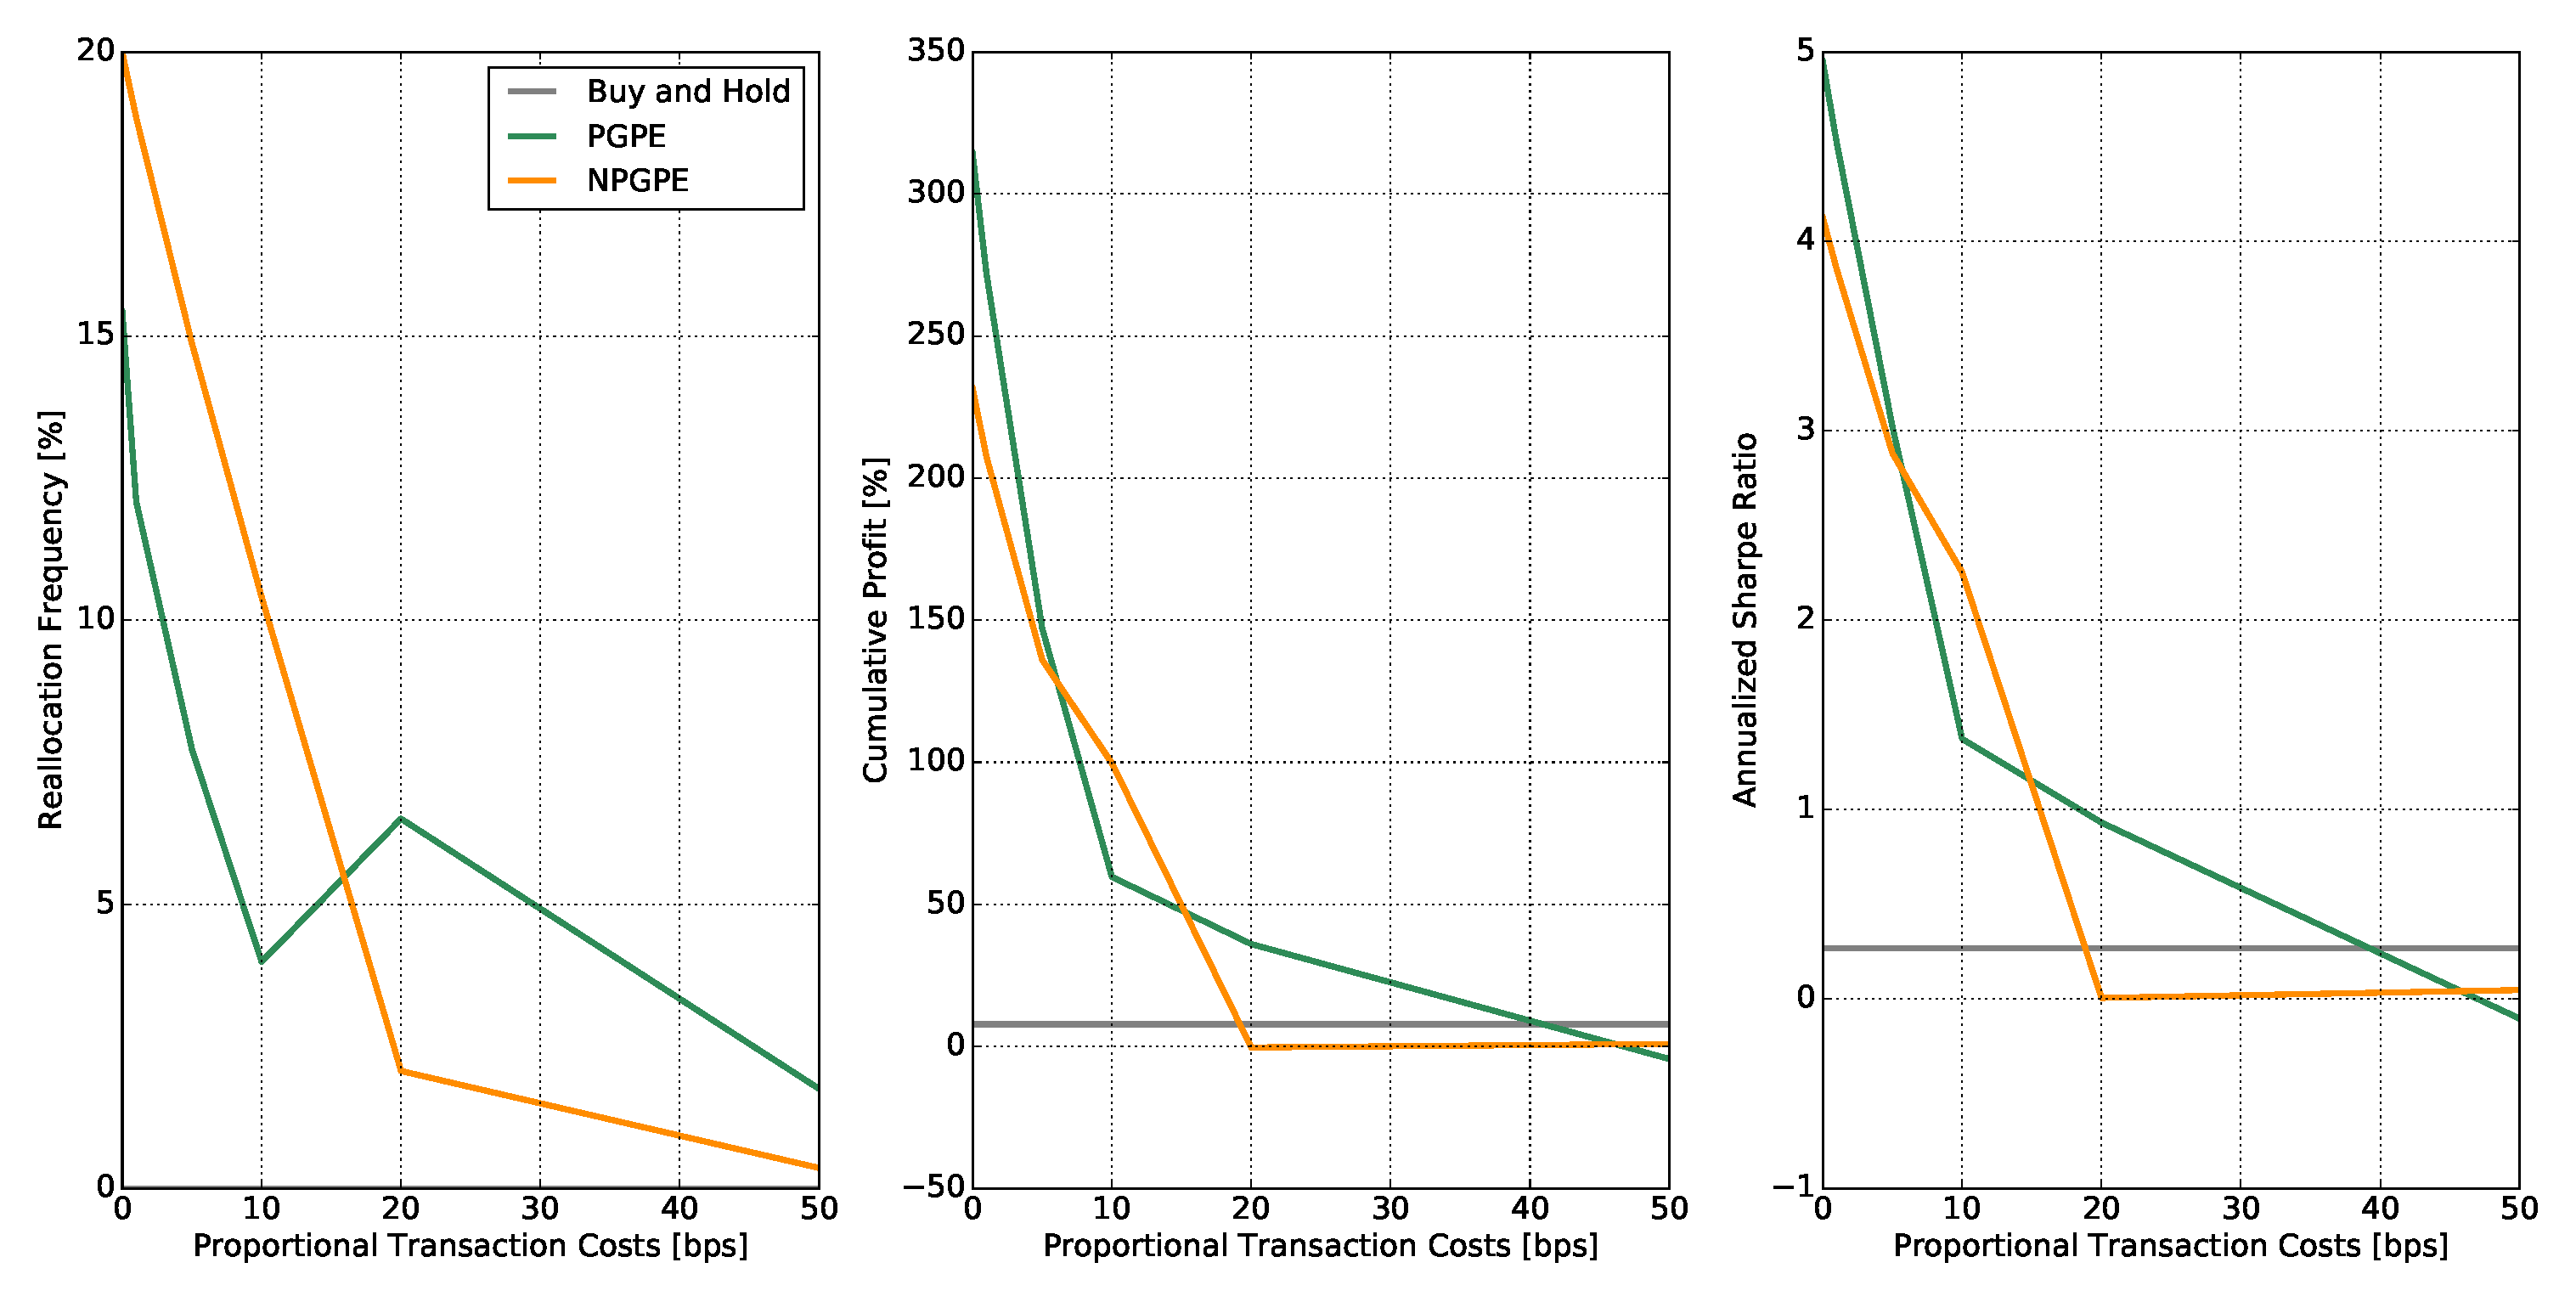
\includegraphics[height=6cm,width=1.0\textwidth]{Images/6_2_impact_transaction_costs}
	\caption[Proportional transaction costs and risk-neutral strategies]{Impact of proportional transaction costs on the trading strategies learned by PGPE and NPGPE.}
	\label{fig:impact_transaction_costs}
\end{figure}
As expected, the frequency of reallocation for both strategies quickly drops to zero as the transaction costs increase, converging to the profitable buy and hold strategy. It is peculiar that the reallocation frequency for the PGPE strategy initially drops more quickly than for the NPGPE strategy, but then slows down and even increases when $\delta_P = 20$ bps. In summary, both algorithms are able to identify reallocation as the cause for lower rewards and to subsequently reduce the rate of reallocation. However, it seems that both algorithms prescribe a zero return buy and hold strategy on the risk-free asset, instead of the more profitable buy and hold strategy on the risky asset.\\
Figure \ref{fig:impact_short_selling_fees} shows the impact of short-selling fees on the trading strategies learned by PGPE and NPGPE. Both algorithms behave as expected, displaying a progressive reduction of the frequency of short positions as the fees increase. For large values of short-selling fees, both strategies converge to the profitable buy and hold strategy, which completely avoids paying the fees. In particular, PGPE quickly replicates the buy and hold strategy. On the other hand, NPGPE is not able to exactly reproduce the buy and hold strategy but it seems to converge to it for very large values of the short-selling fee. 
\begin{figure}[t!]
	\centering
	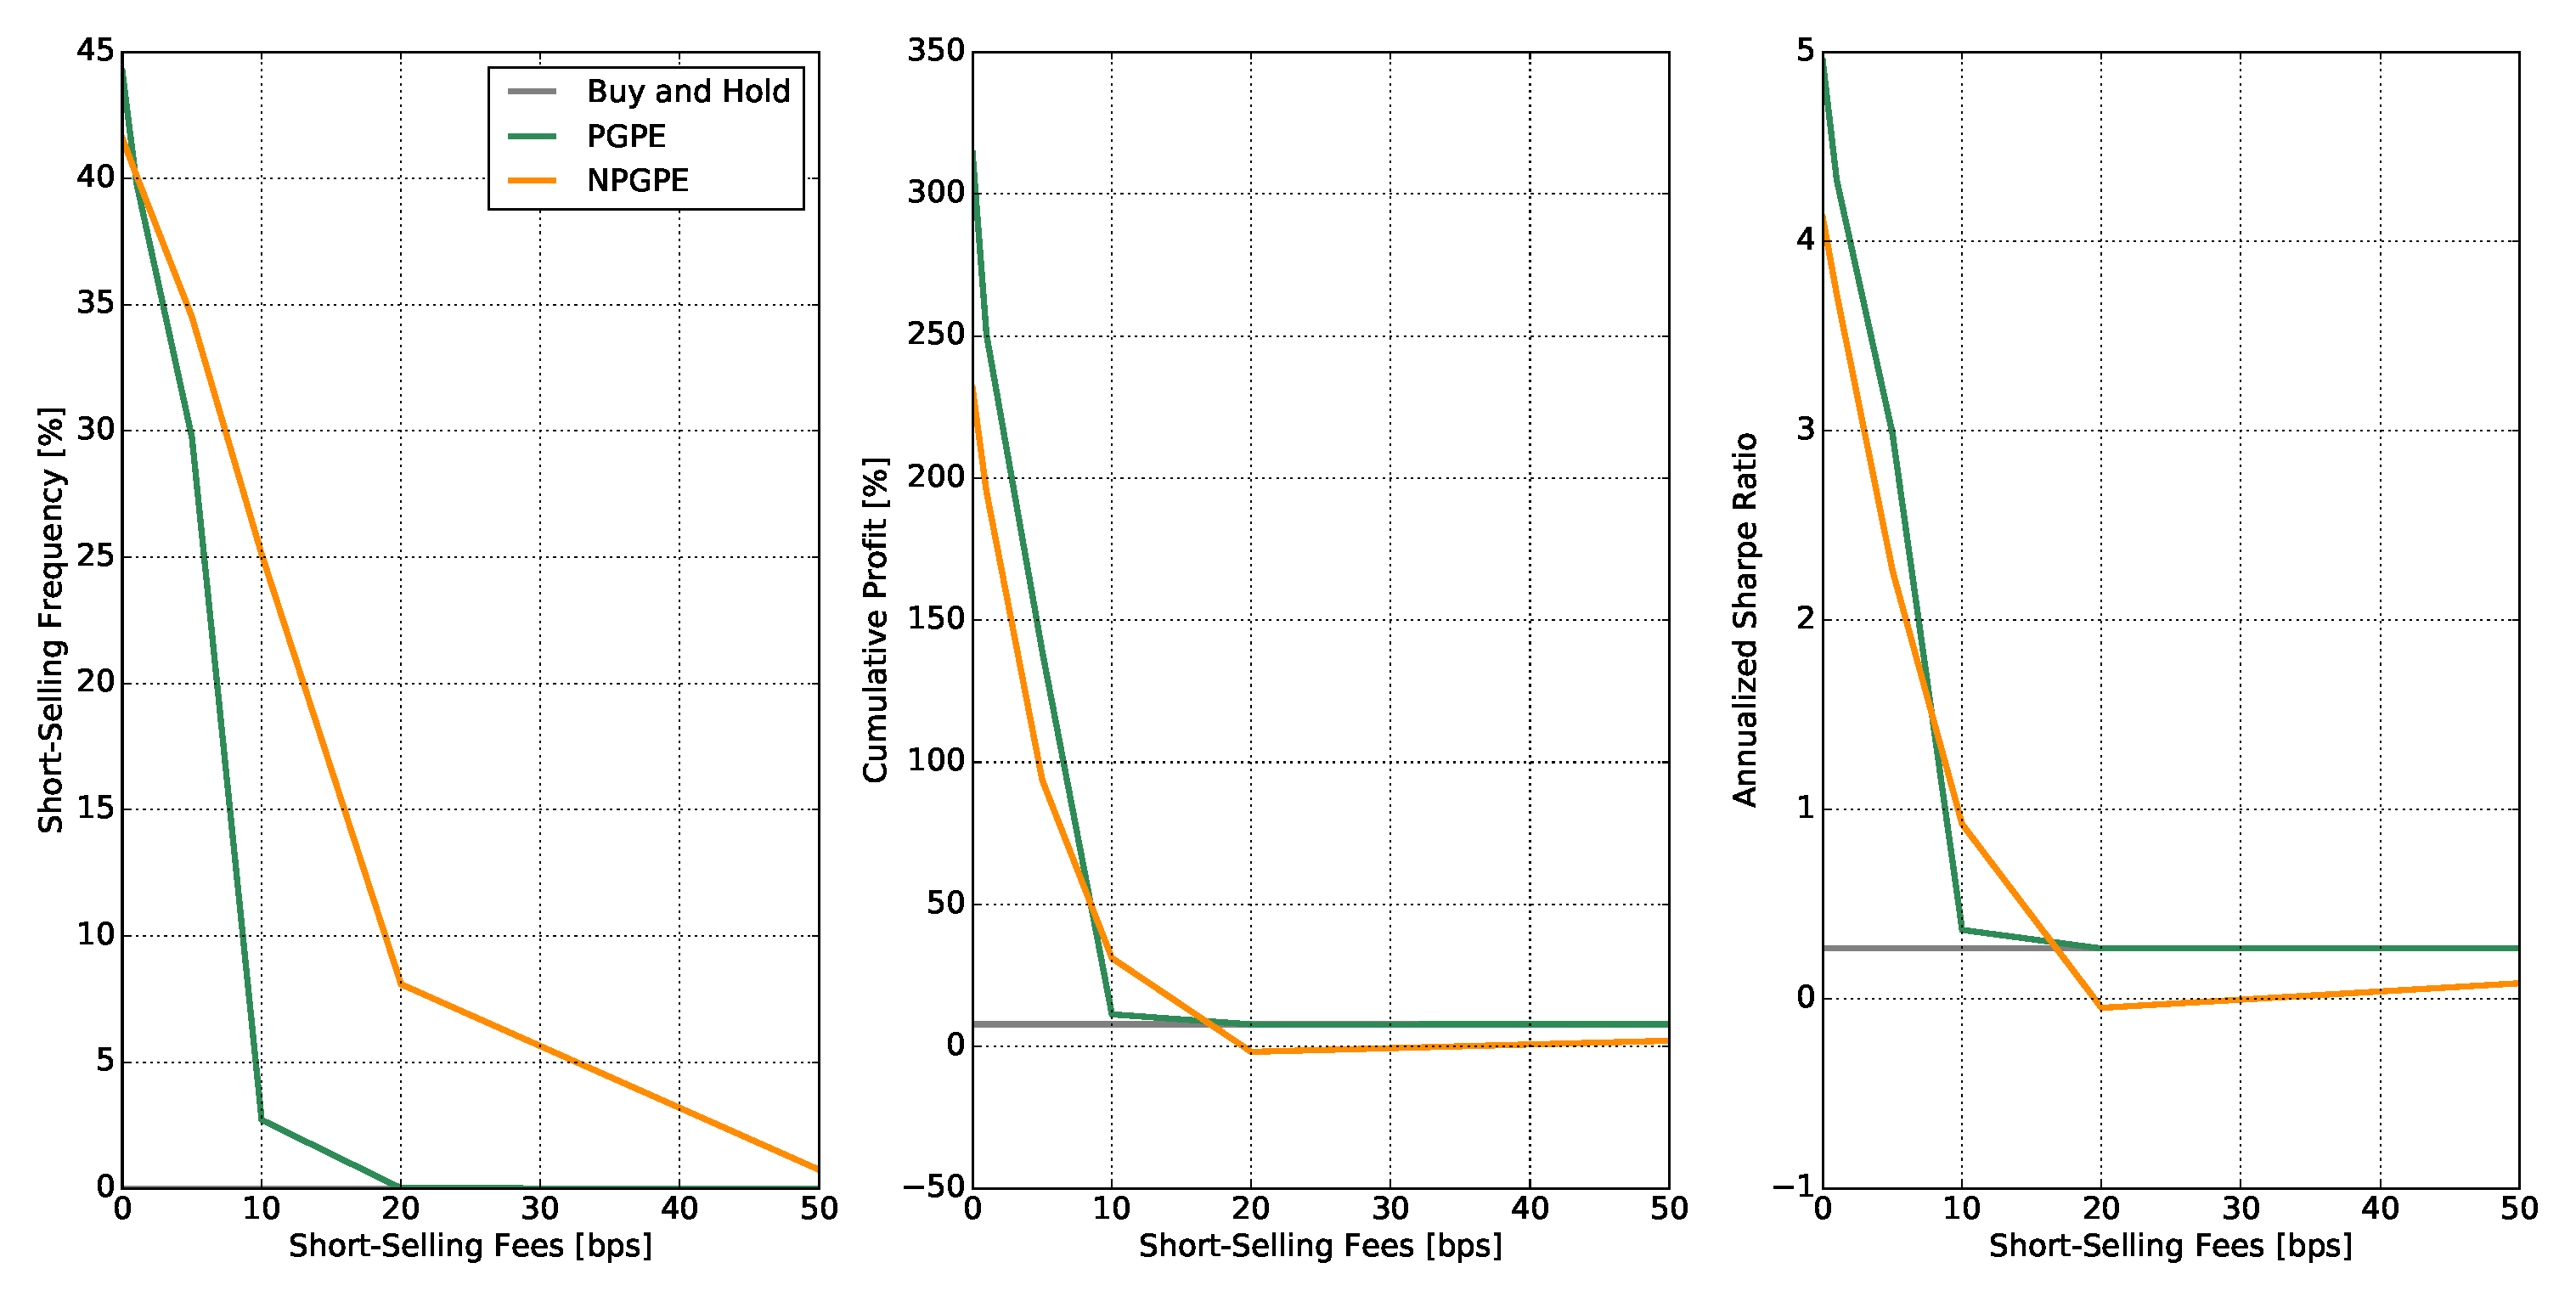
\includegraphics[height=6cm,width=1.0\textwidth]{Images/6_3_impact_short_selling_fees}
	\caption[Short-selling fees and risk-neutral strategies]{Impact of short-selling fees on the trading strategies learned by PGPE and NPGPE.}
	\label{fig:impact_short_selling_fees}
\end{figure}

\subsection{Risk-Sensitive Framework}
In this section we present the results in the risk-sensitive framework, in which the learning algorithms optimize the Sharpe ratio of the policy. Figure \ref{fig:single_synthetic_sensitive_convergence} shows the learning curves for the three risk-sensitive algorithms RSPGPE and RSNPGPE. We observe that the natural-gradient algorithm converges to a larger Sharpe ratio compared to the non-natural algorithm, which converges very quickly to a suboptimal policy. It is interesting that the risk-sensitive algorithms converge faster than their risk-neutral counterparts. Surprisingly, the strategies learned by the risk-sensitive algorithms have smaller Sharpe ratio than those learned in the risk-neutral version, in which we don't explicitly control risk. We still don't have a clear explanation for this counter-intuitive behavior. A first hypothesis is that, for the stationary dynamics considered to generate the price series, the optimal policy in the risk-neutral sense also minimize risk, but directly optimizing the Sharpe ratio is more difficult as more parameters and noise are involved in the learning process. Further research should be carried out to investigate this issue in more depth. Figure \ref{fig:single_synthetic_sensitive_performance} shows the backtest performances for the risk-sensitive trading strategies, which both outperform the simple buy-and-hold strategy. More statistics are reported in Table \ref{tab:single_synthetic_sensitive_performance}. We notice that, contrarily to the risk-neutral setting, NPGPE performs better than PGPE with respect to all the performance measures. In particular, the policy learned by PGPE takes much less short positions, which negatively impacts the performance of the strategy.

\begin{figure}[t!]
	\centering
	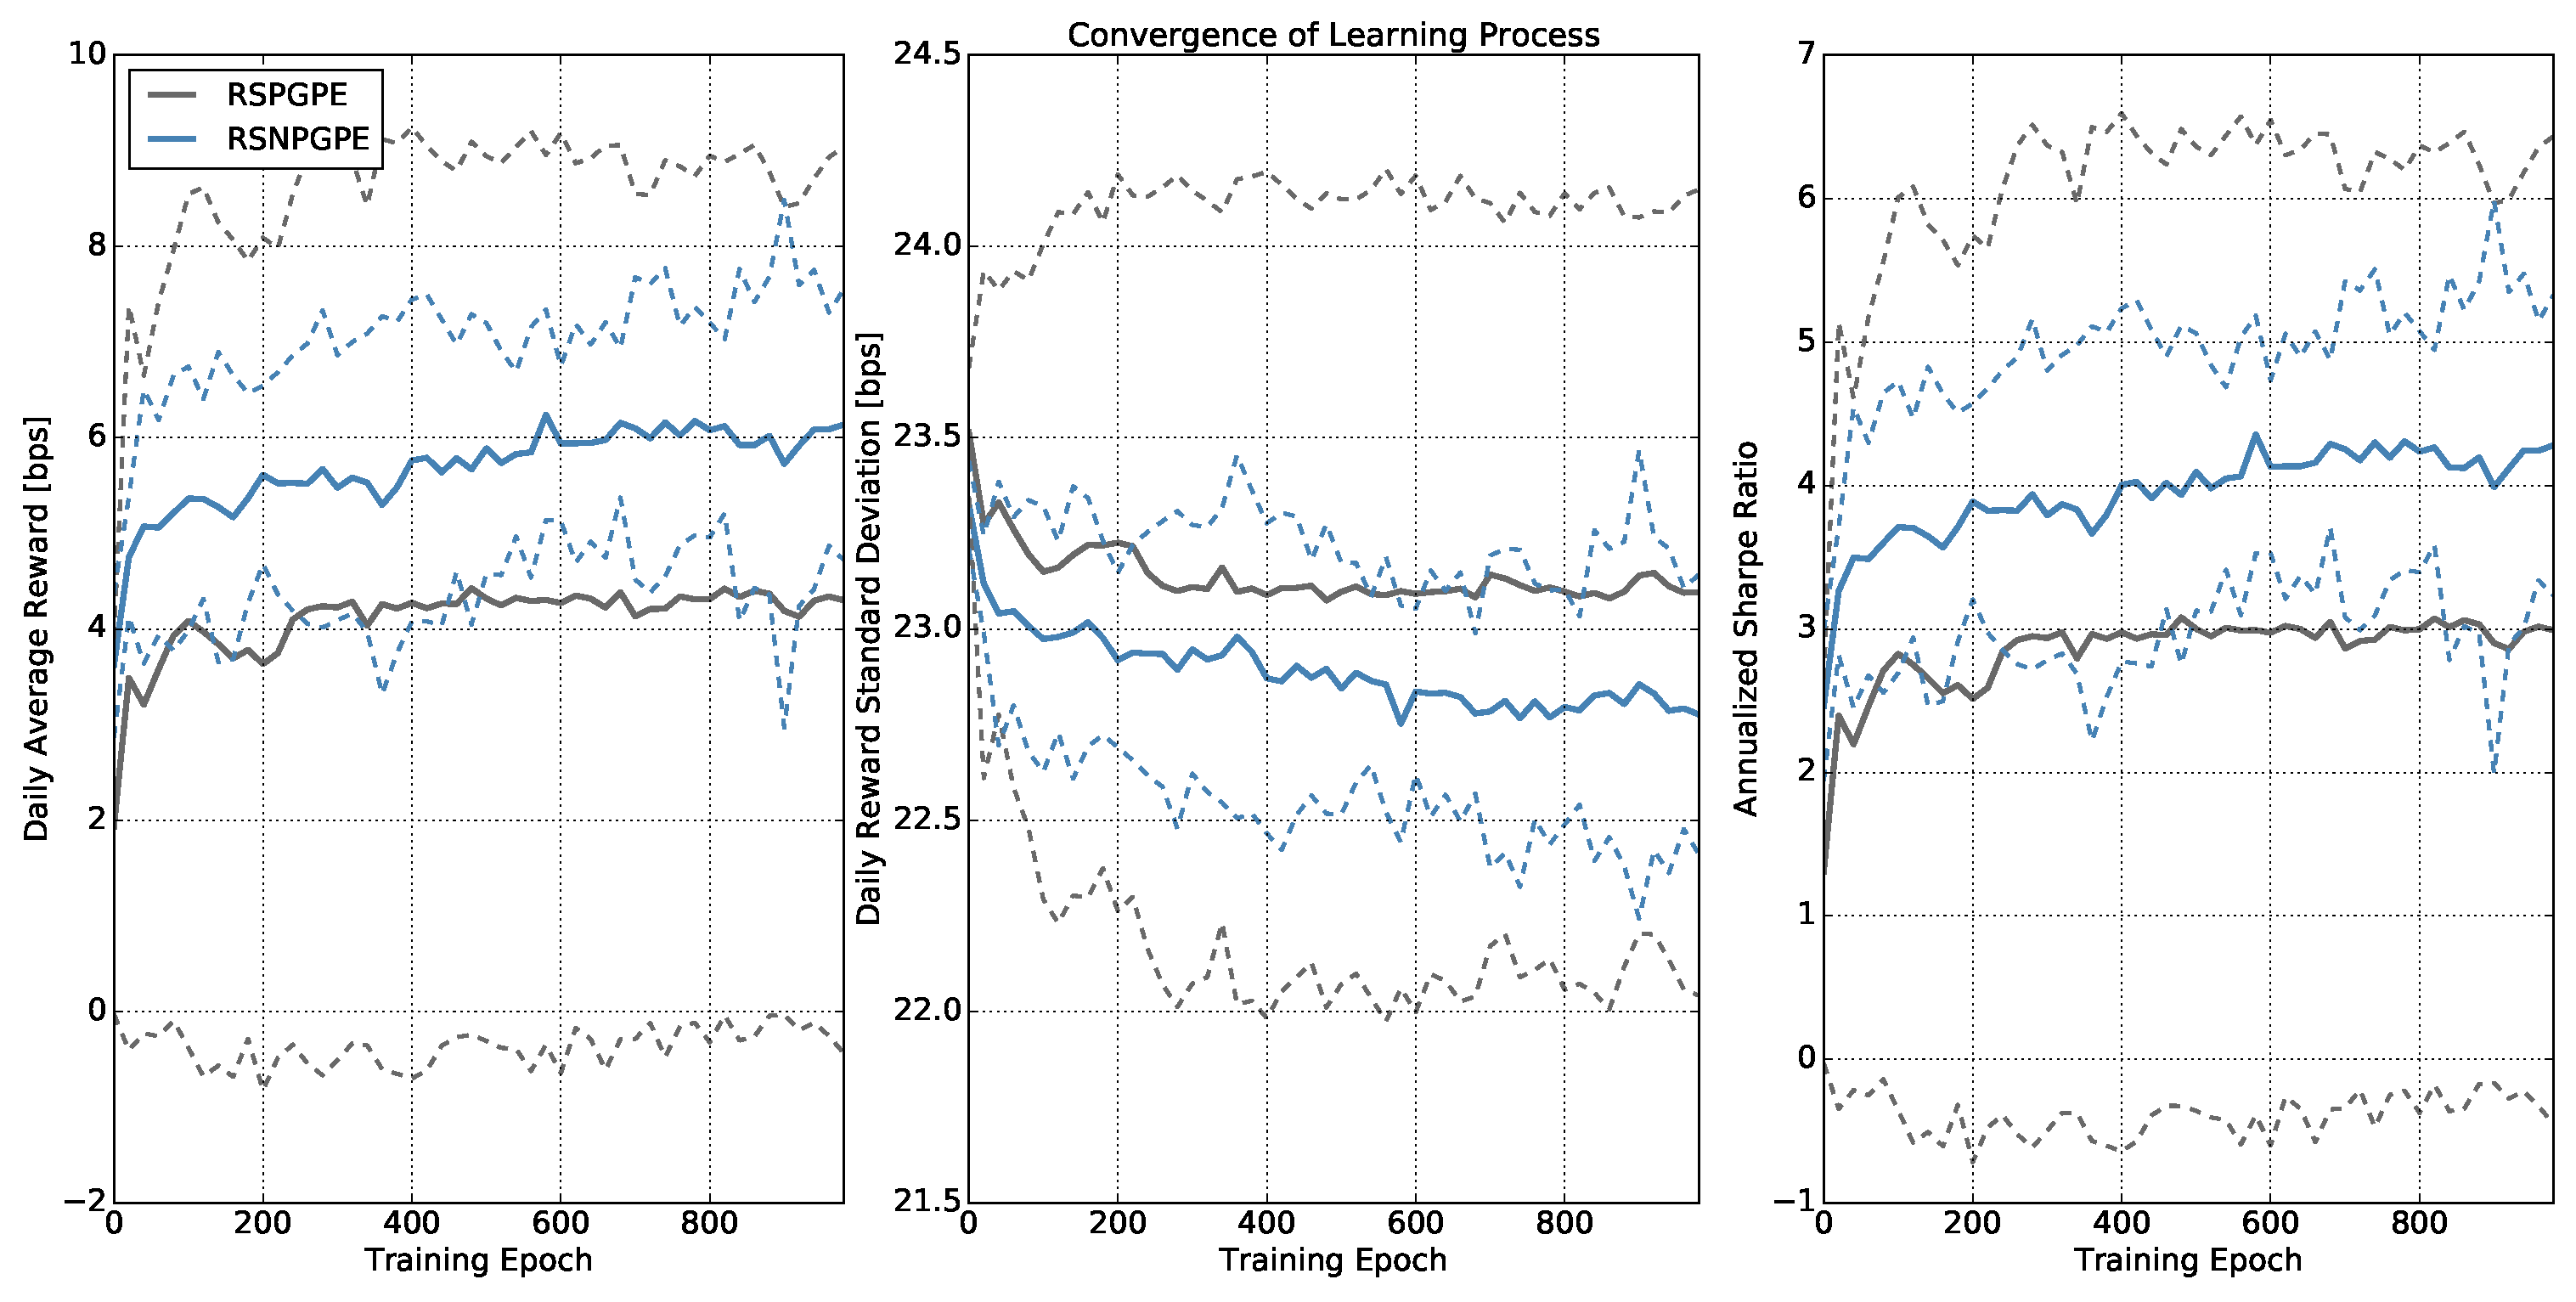
\includegraphics[height=6cm,width=1.0\textwidth]{Images/8_4_single_synthetic_sensitive_convergence}
	\caption[Risk-sensitive learning process for one synthetic risky asset]{Risk-sensitive learning process for the asset allocation problem with one synthetic risky asset.}
	\label{fig:single_synthetic_sensitive_convergence}
\end{figure}

\begin{figure}[t!]
	\centering
	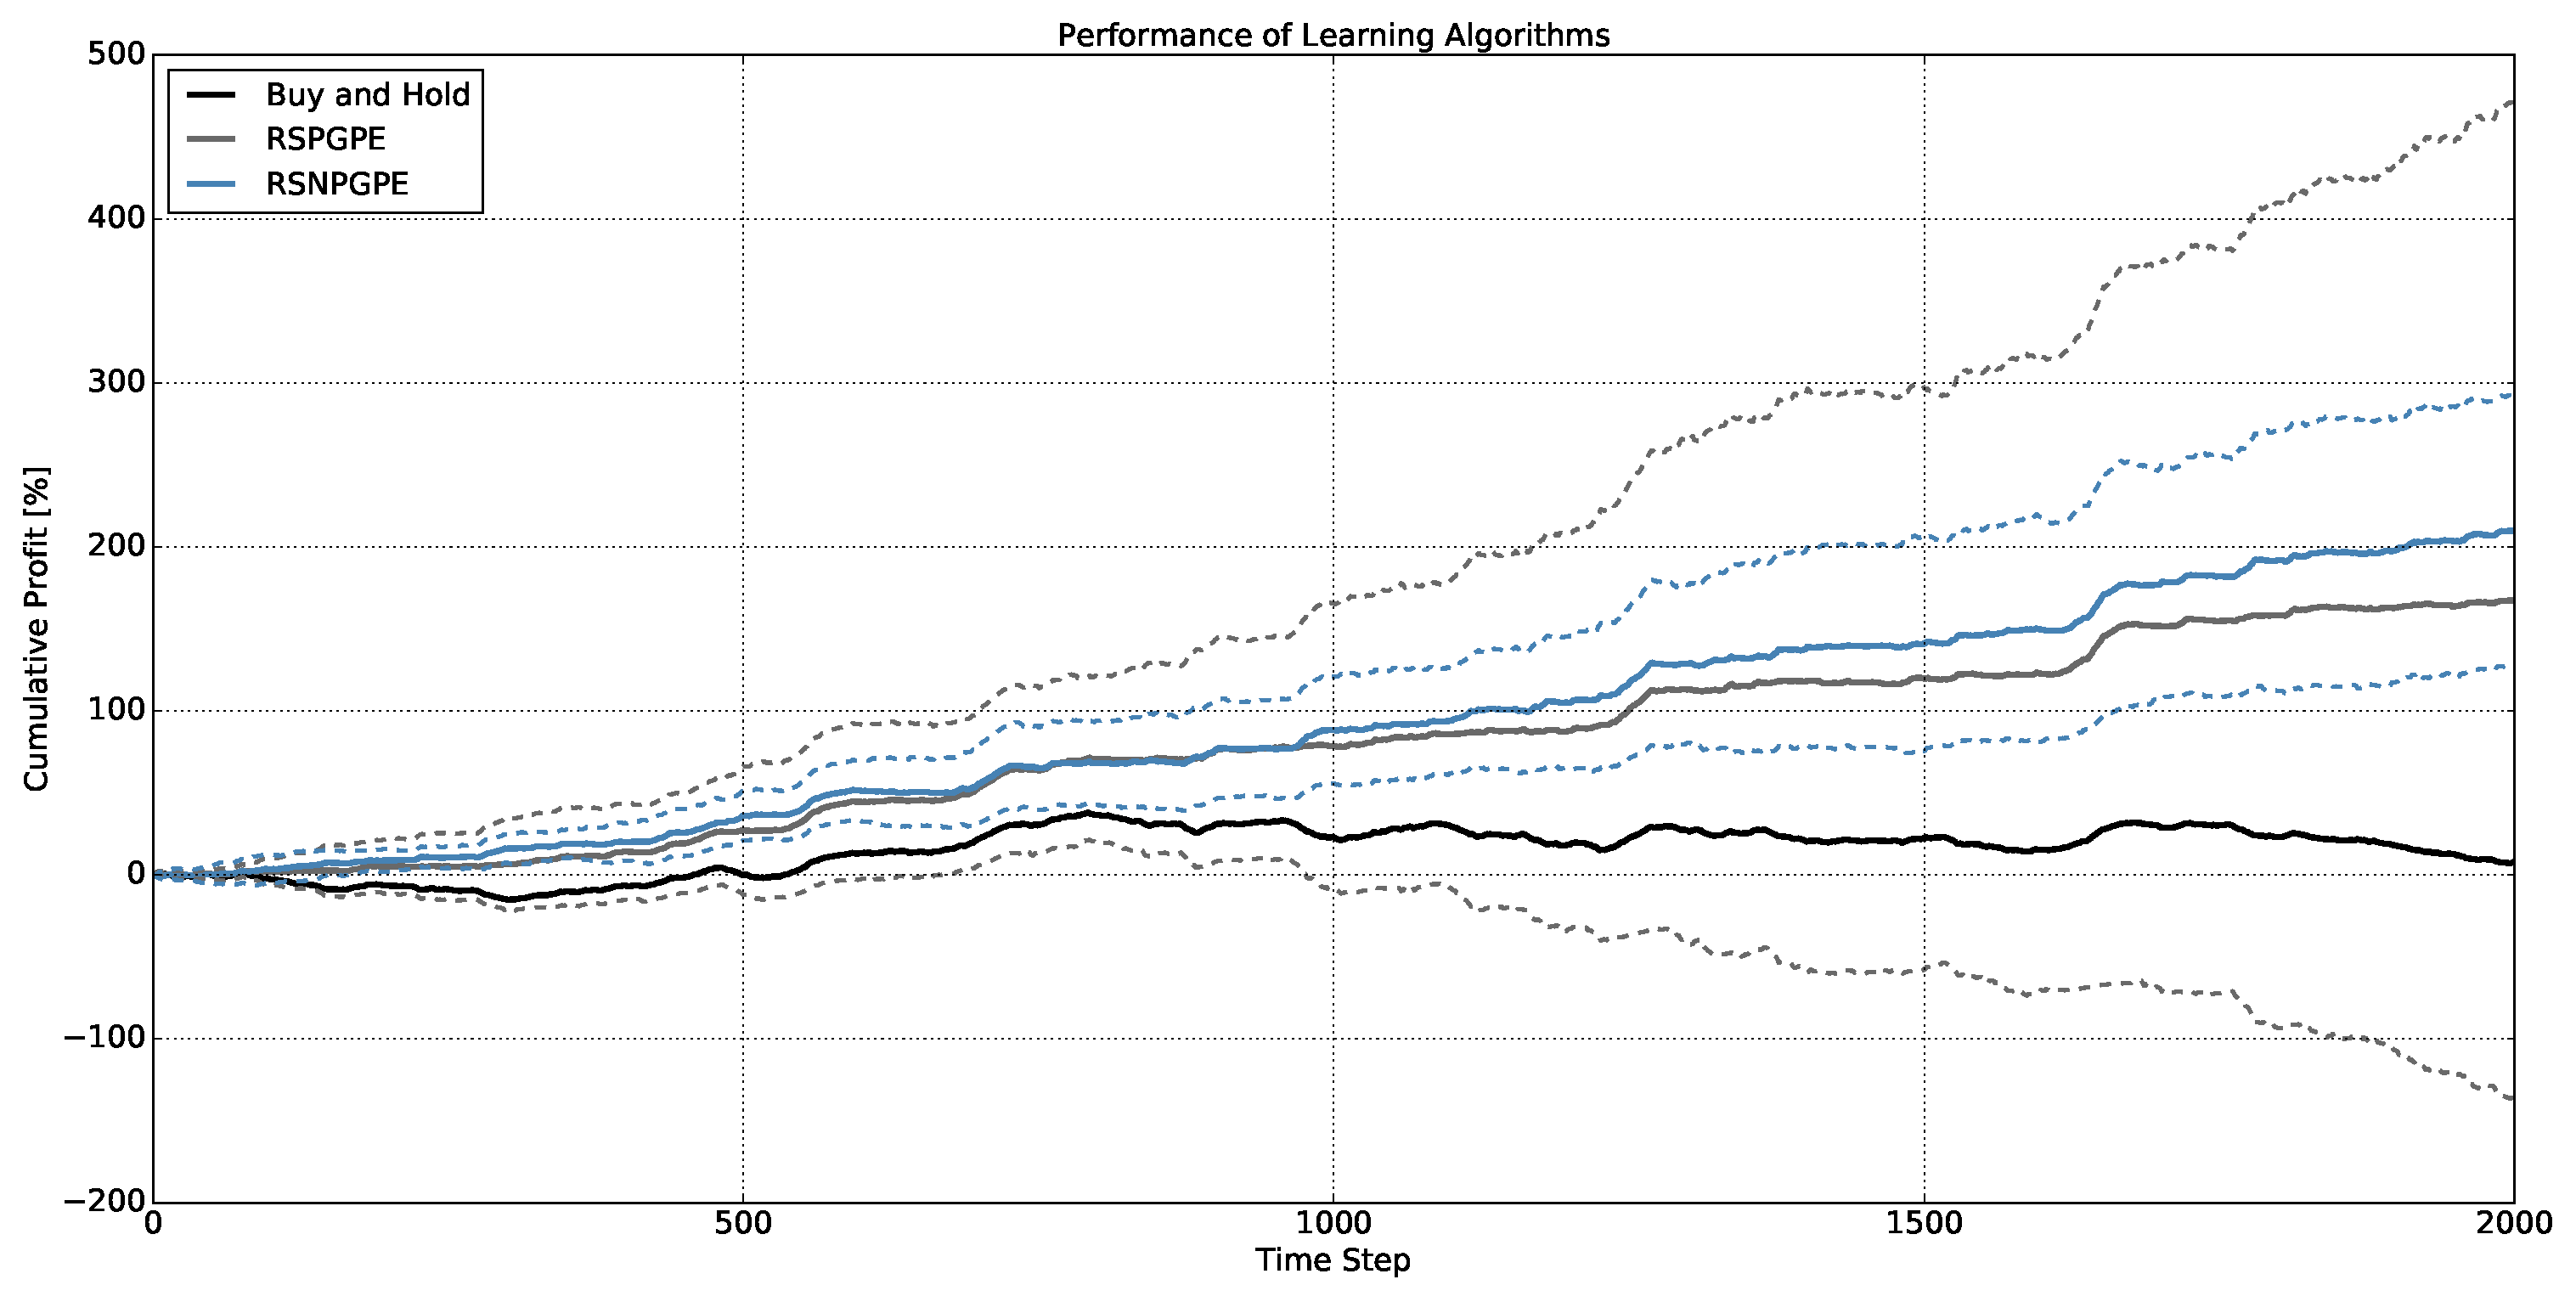
\includegraphics[width=1.0\textwidth]{Images/8_5_single_synthetic_sensitive_performance}
	\caption[Backtest performance with one synthetic risky asset]{Backtest performance of the risk-sensitive trading strategies for the asset allocation problem with one synthetic risky asset.}
	\label{fig:single_synthetic_sensitive_performance}
\end{figure}

\begin{table}[h!]
\centering
\begin{tabular}{@{}lrrr@{}}
\toprule
                  & Buy and Hold & RSPGPE   & RSNPGPE  \\ \midrule
Total Return      & 7.81\%       & 82.29\%  & 219.81\% \\
Daily Sharpe      & 0.27         & 1.95     & 3.97     \\
Monthly Sharpe    & 0.19         & 1.19     & 2.84     \\
Yearly Sharpe     & 0.23         & 0.67     & 1.71     \\
Max Drawdown      & -22.35\%     & -11.56\% & -3.60\%  \\
Avg Drawdown      & -1.75\%      & -1.00\%  & -0.47\%  \\
Avg Up Month      & 2.87\%       & 2.65\%   & 2.41\%   \\
Avg Down Month    & -2.58\%      & -1.48\%  & -0.71\%  \\
Win Year \%       & 40.00\%      & 76.00\%  & 100.00\% \\
Win 12m \%        & 56.36\%      & 87.45\%  & 100.00\% \\
Reallocation Freq & 0.00\%       & 15.50\%  & 28.00\%  \\
Short Freq        & 0.00\%       & 16.17\%  & 45.77\%  \\ \bottomrule
\end{tabular}
\caption[Backtest statistics for risk-sensitive learning with one synthetic risky asset]{Backtest statistics of the risk-sensitive trading strategies for the asset allocation problem with one synthetic risky asset.}
\label{tab:single_synthetic_sensitive_performance}
\end{table}

\subsubsection{Risk-Neutral vs. Risk-Sensitive}
The risk-neutral NPGPE and the risk-sensitive NPGPE strategies achieve very similar backtest performances. A natural question that arises is if the two algorithms are actually learning the same policy. The two versions of the NPGPE algorithm are compared in Table \ref{tab:comparison_NPGPE}. The statistics for the two algorithms are similar. Again, we point out the counter-intuitive fact that risk-neutral version produces higher Sharpe ratios, even if it is not the quantity directly being optimized. On the other hand, the risk-sensitive version seems to perform slightly better in terms of drawdowns. The most interesting feature is the different behavior of the two policies in terms of reallocation and short-selling frequencies. The risk-sensitive policy reshuffle the portfolio more frequently than the risk-neutral policy, also resorting more often to short positions. This shows that the policies learned by the two algorithms are actually different, leading however to very similar performances. 

\begin{table}[t!]
\centering
\begin{tabular}{@{}lrr@{}}
\toprule
                  & NPGPE   & RSNPGPE  \\ \midrule
Total Return      & 231.63\%  & 219.81\% \\
Daily Sharpe      & 4.13     & 3.97     \\
Monthly Sharpe    & 2.90     & 2.84     \\
Yearly Sharpe     & 1.55     & 1.71     \\
Max Drawdown      & -3.72\% & -3.60\%  \\
Avg Drawdown      & -0.49\%  & -0.47\%  \\
Avg Up Month      & 2.47\%   & 2.41\%   \\
Avg Down Month    & -0.73\%  & -0.71\%  \\
Win Year \%       & 98.00\%  & 100.00\% \\
Win 12m \%        & 100.00\%  & 100.00\% \\
Reallocation Freq & 19.99\%  & 28.00\%  \\
Short Freq        & 41.59\%  & 45.77\%  \\ \bottomrule
\end{tabular}
\caption{Comparison of NPGPE and RSNPGPE for the asset allocation problem with one synthetic risky asset.}
\label{tab:omparison_NPGPE}
\end{table}

\subsubsection{Impact of Transaction Costs}
Once again we study the sensitivity of the trading strategies learned by RSPGPE and RSNPGPE with respect to transaction costs and short-selling fees. Intuitively, as the transaction costs increase we expect a progressive reduction of the frequency of reallocation and of shorting the risky asset.\\
Figure \ref{fig:8_6_impact_transaction_costs_RS} shows the impact of proportional transaction costs on the trading strategies learned while Figure \ref{fig:8_7_impact_short_selling_fees_RS} shows that of short-selling fees. We observe that RSNPGPE quickly converge to the profitable Buy and Hold strategy in both situations. This was not the case in the risk-neutral framework, where NPGPE underperformed the benchmark when the transaction costs were large enough. Disappointingly, RSPGPE doesn't adapt to the increasing transaction costs as expected, leading to large losses. While, the reallocation frequency decreases (but not enough to avoid a loss), the frequency of short position appears to be independent of the short-selling fees. Further analysis is necessary to explain this unexpected behavior of RSPGPE which is not observed in the risk-neutral framework. 

\begin{figure}[t!]
\centering
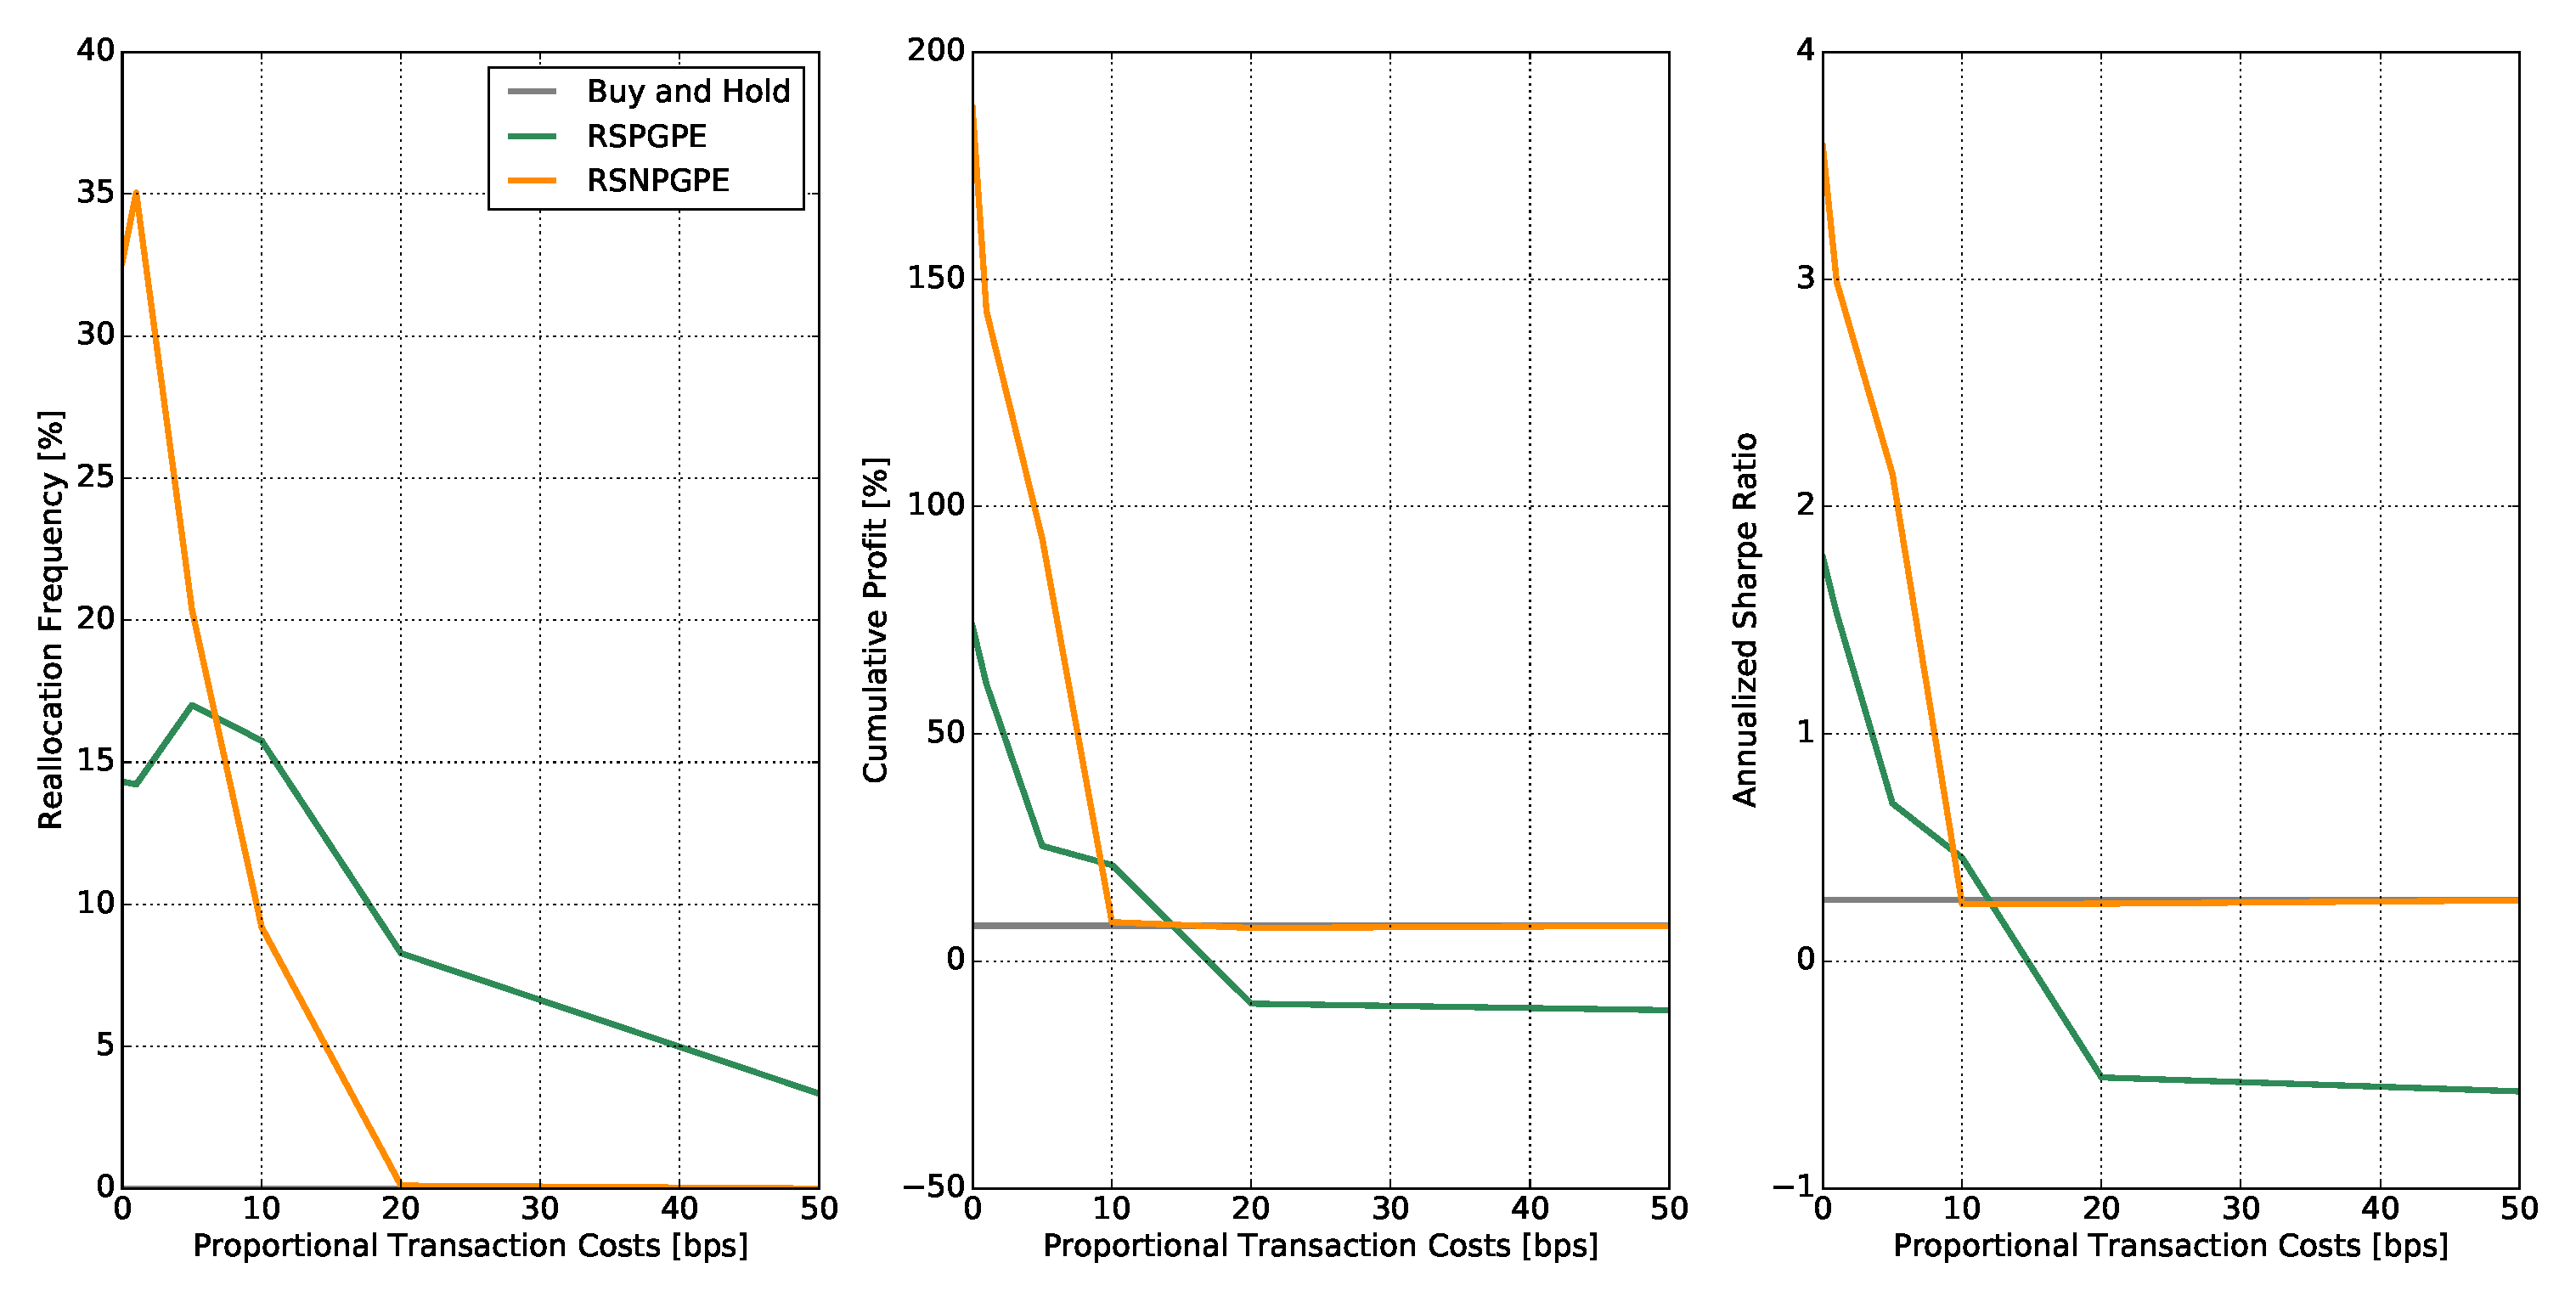
\includegraphics[height=6cm,width=1\linewidth]{Images/8_6_impact_transaction_costs_RS}
\caption[Proportional transaction costs and risk-sensitive strategies]{Impact of proportional transaction costs on the trading strategies learned by RSPGPE and RSNPGPE.}
\label{fig:8_6_impact_transaction_costs_RS}
\end{figure}

\begin{figure}[t!]
\centering
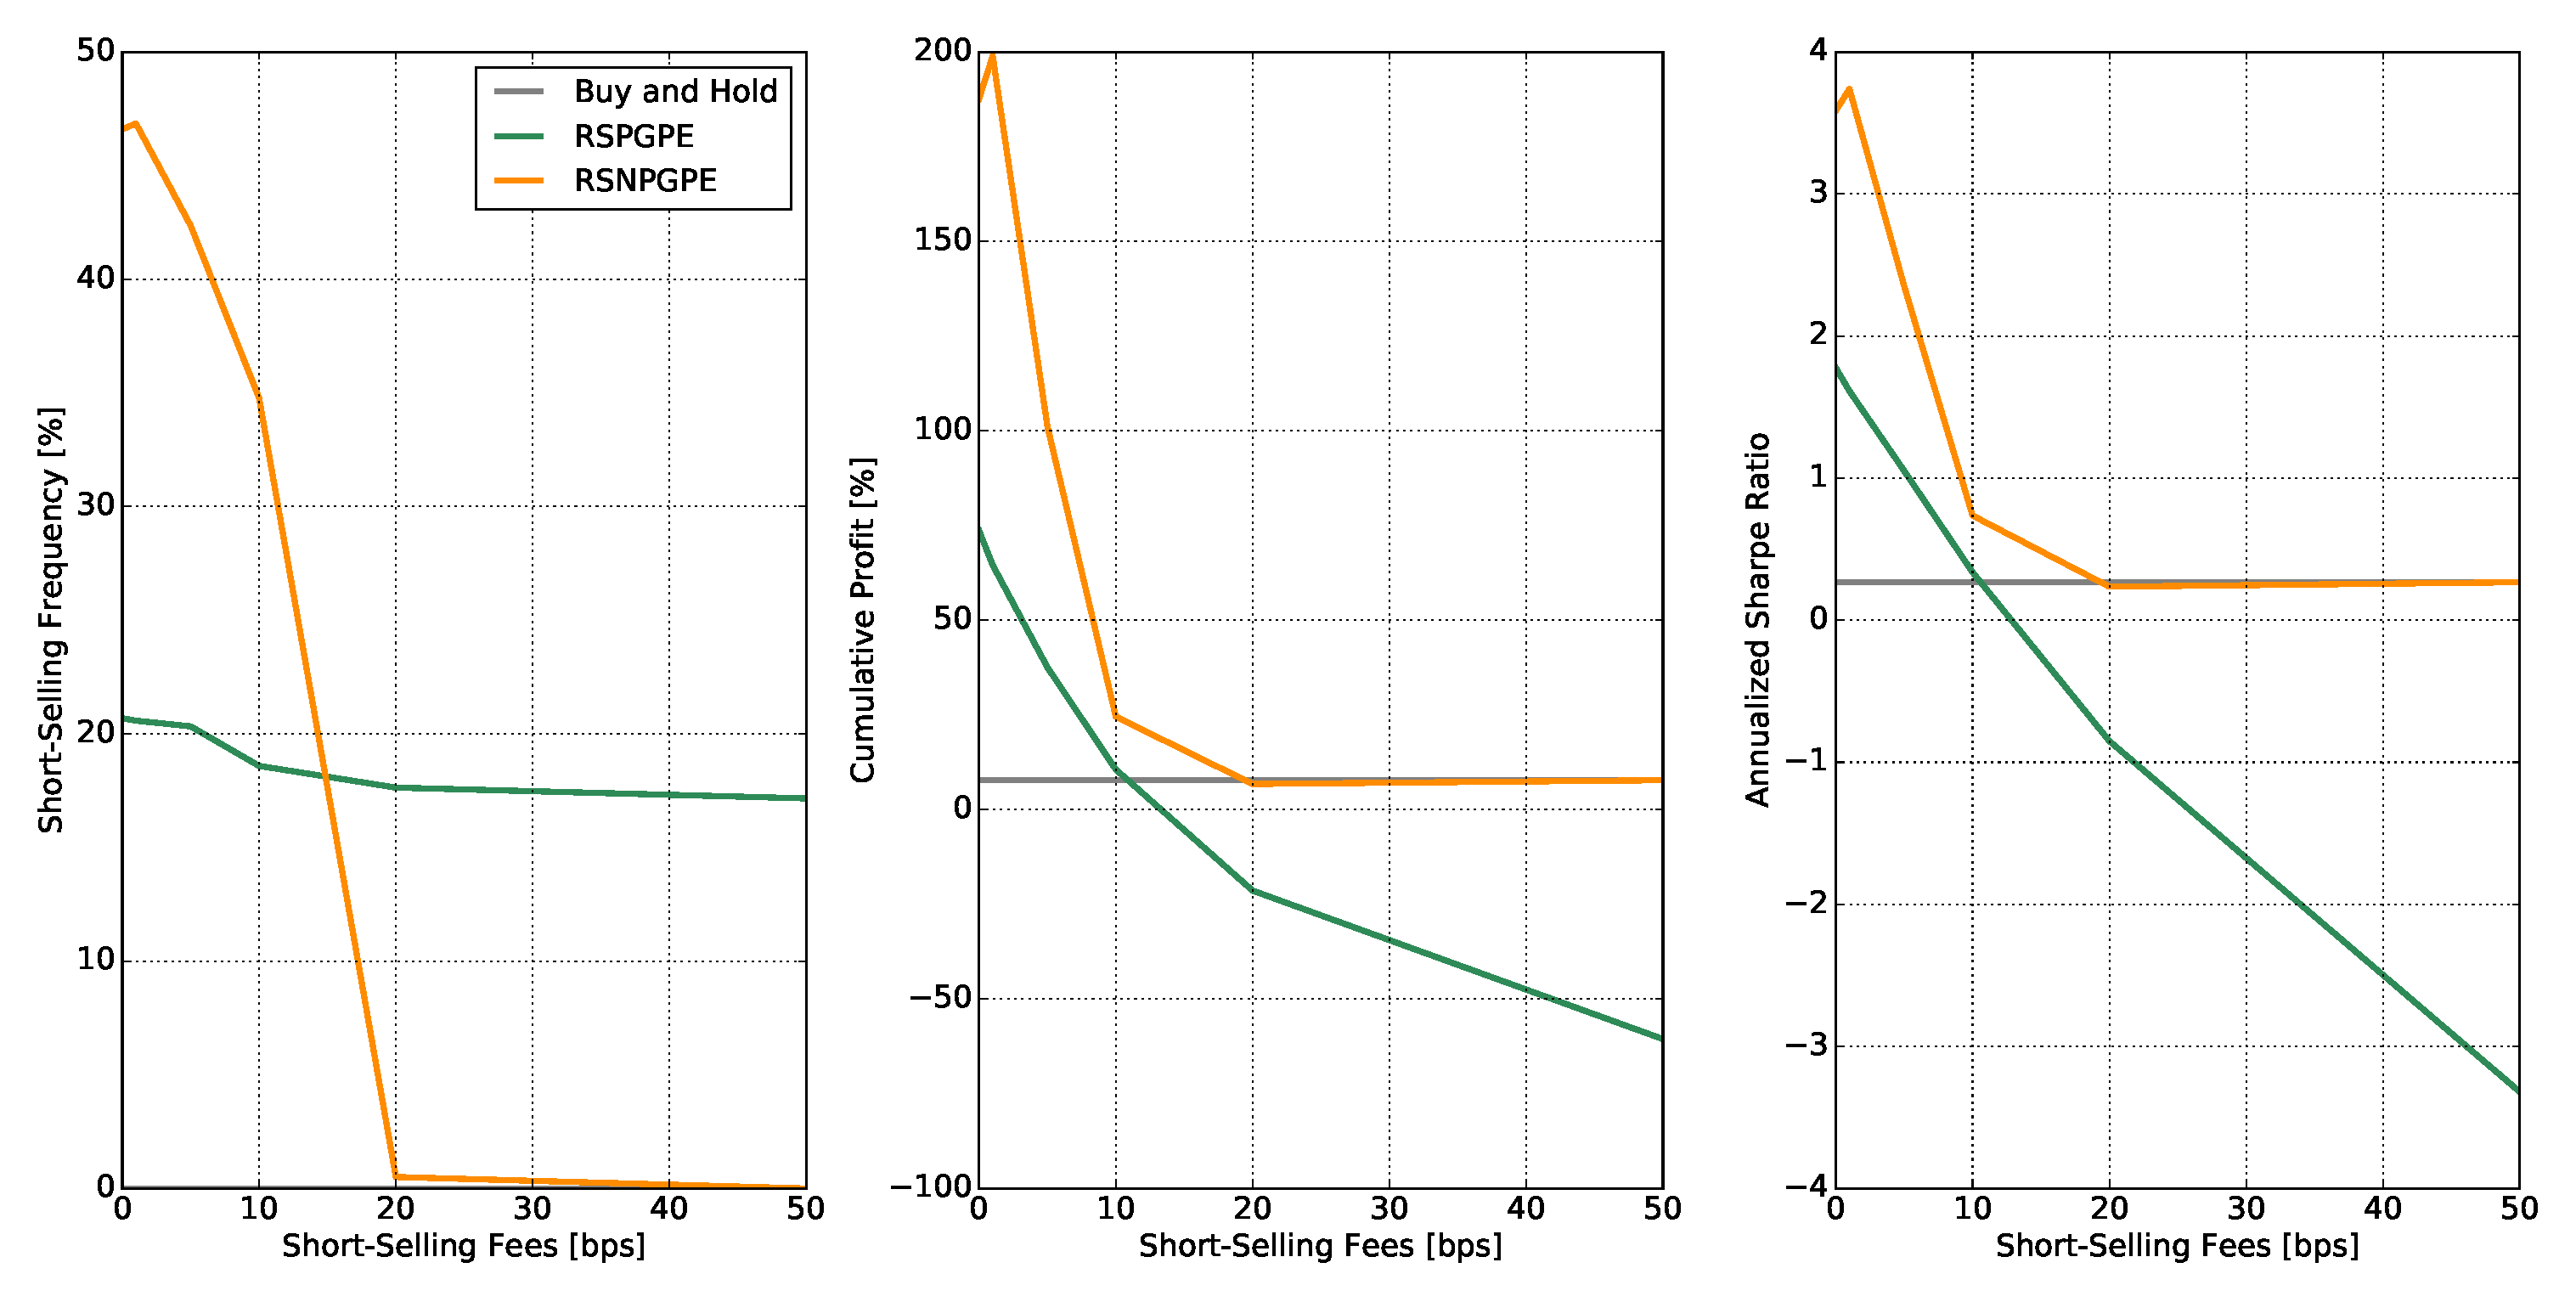
\includegraphics[height=6cm,width=1\linewidth]{Images/8_7_impact_short_selling_fees_RS}
\caption[Short-selling fees and risk-sensitive strategies]{Impact of short-selling fees on the trading strategies learned by RSPGPE and RSNPGPE.}
\label{fig:8_7_impact_short_selling_fees_RS}
\end{figure}

\clearpage
\section{Historic Risky Asset}
In this section we discuss the attempt to apply the algorithms above to an historical price series. As a test case, we considered a stock of Banca Monte dei Paschi di Siena (BMPS IM) as the risky asset. In this case, the algorithms perform poorly and are not able to identify a profitable trading strategy. In some measure, this was expected given the simplicity of the parametric policy considered. When working on historical price series, there are multiple challenges to be addressed. First, it is not clear if the price series contains some patterns that could be traded profitably. This is the central issue of the \gls{EMH} which was discussed in Section \ref{sec:efficient_market_hypothesis}. Now, even if the prices contained a certain degree of predictability, the parametric policy should be sufficiently expressive to capture these patterns. This is clearly an issue of the current state of work, as the policy considered here is so simple that it would be surprising that the policy managed to capture a profitably tradable structure in the prices of a liquid stock. A possible development would be to employ a much more complex parametric policy, such as a neural network, in order to automatically extract more powerful features from the raw price series. Another related issue is the signal-to-noise ratio of financial time-series. 


assuming that the 

the parametric policy 

\begin{figure}[t!]
	\centering
	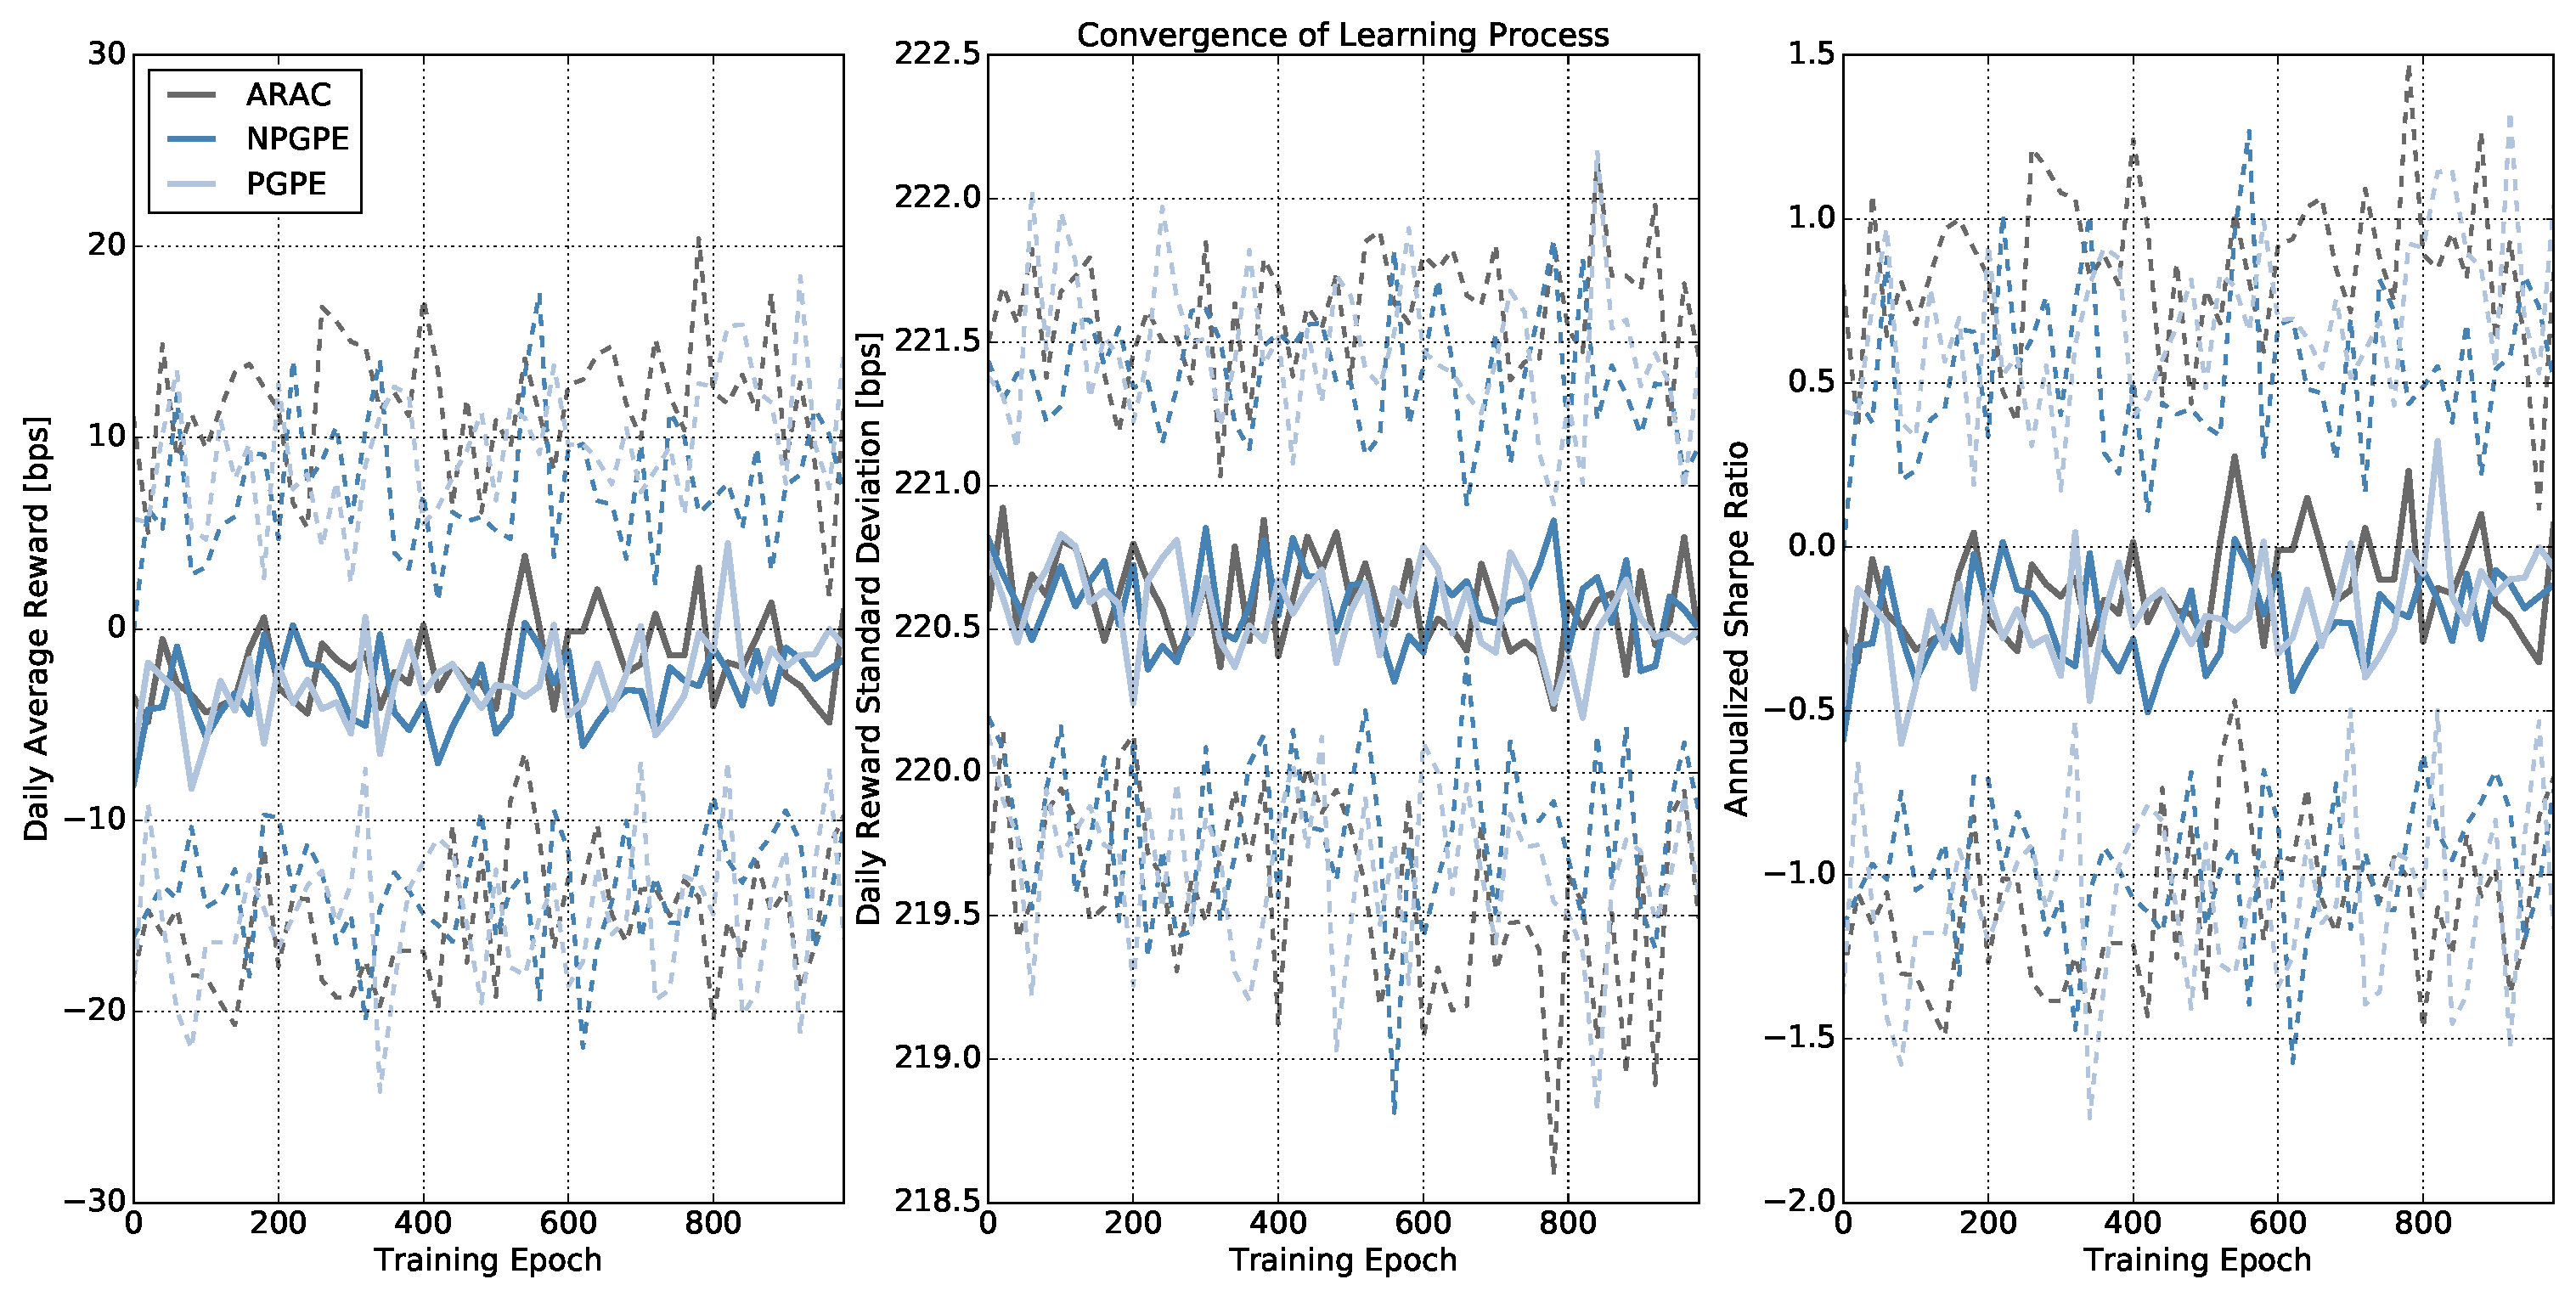
\includegraphics[height=6cm,width=1.0\textwidth]{Images/8_8_single_hist_neutral_convergence}
	\caption[]{}
	\label{fig:}
\end{figure}

\begin{figure}[t!]
	\centering
	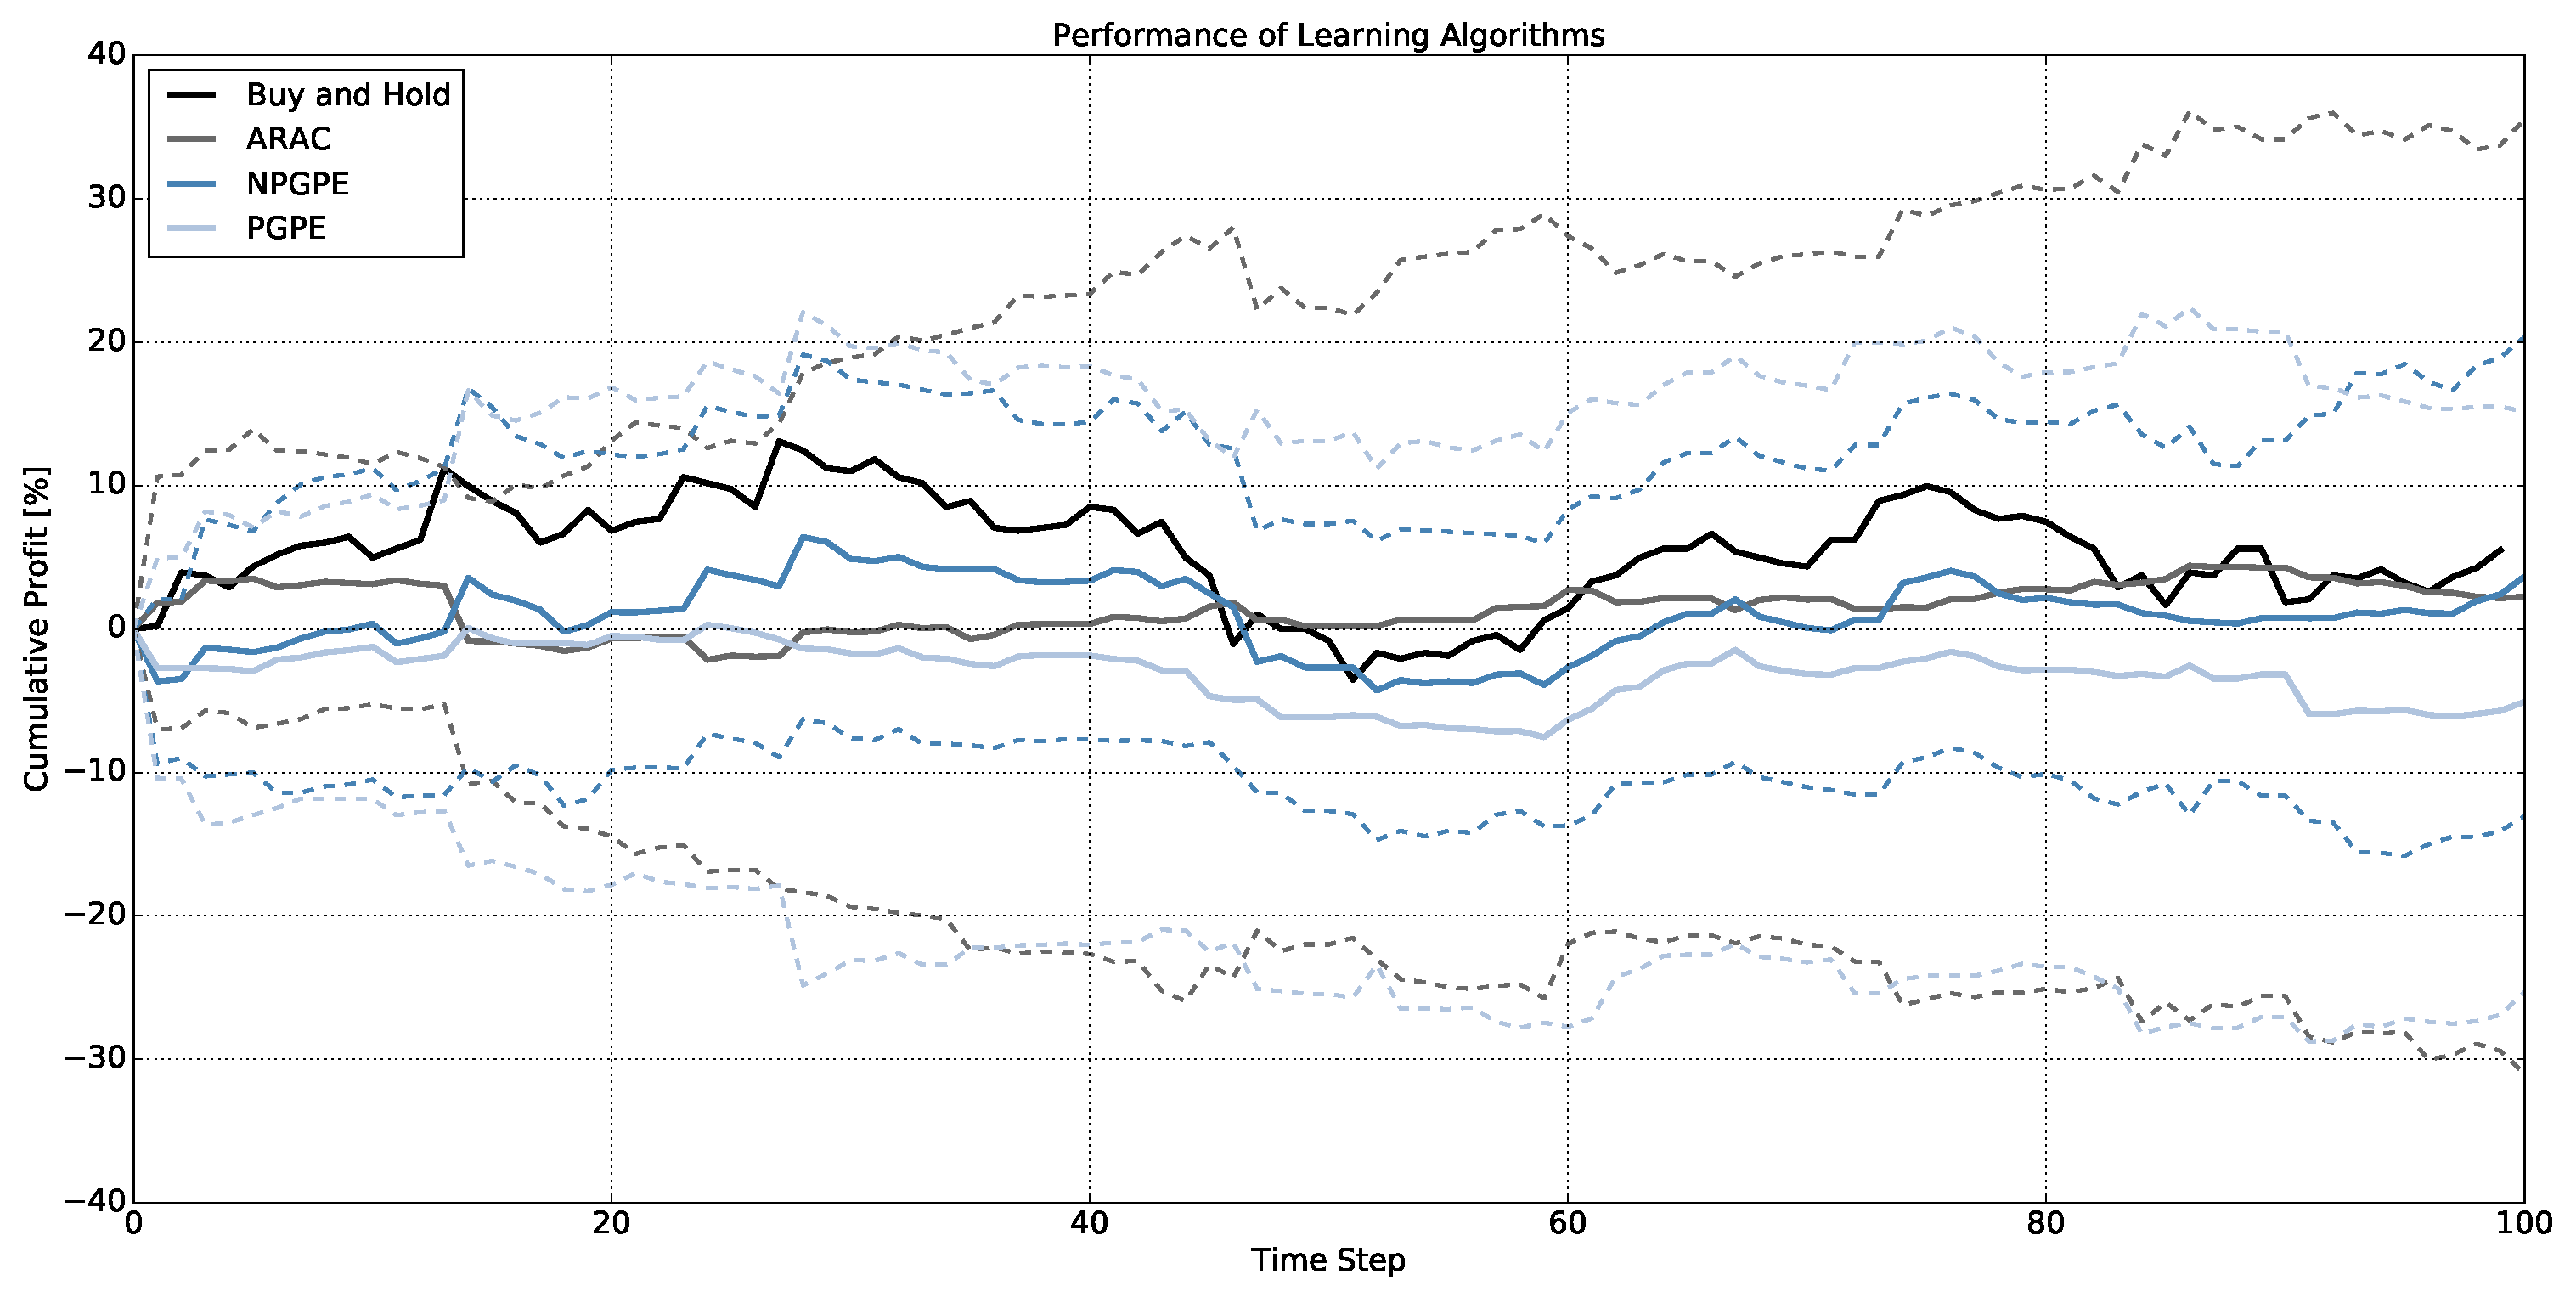
\includegraphics[height=6cm,width=1.0\textwidth]{Images/8_9_single_hist_neutral_performance}
	\caption[]{}
	\label{fig:}
\end{figure}

\begin{figure}[t!]
	\centering
	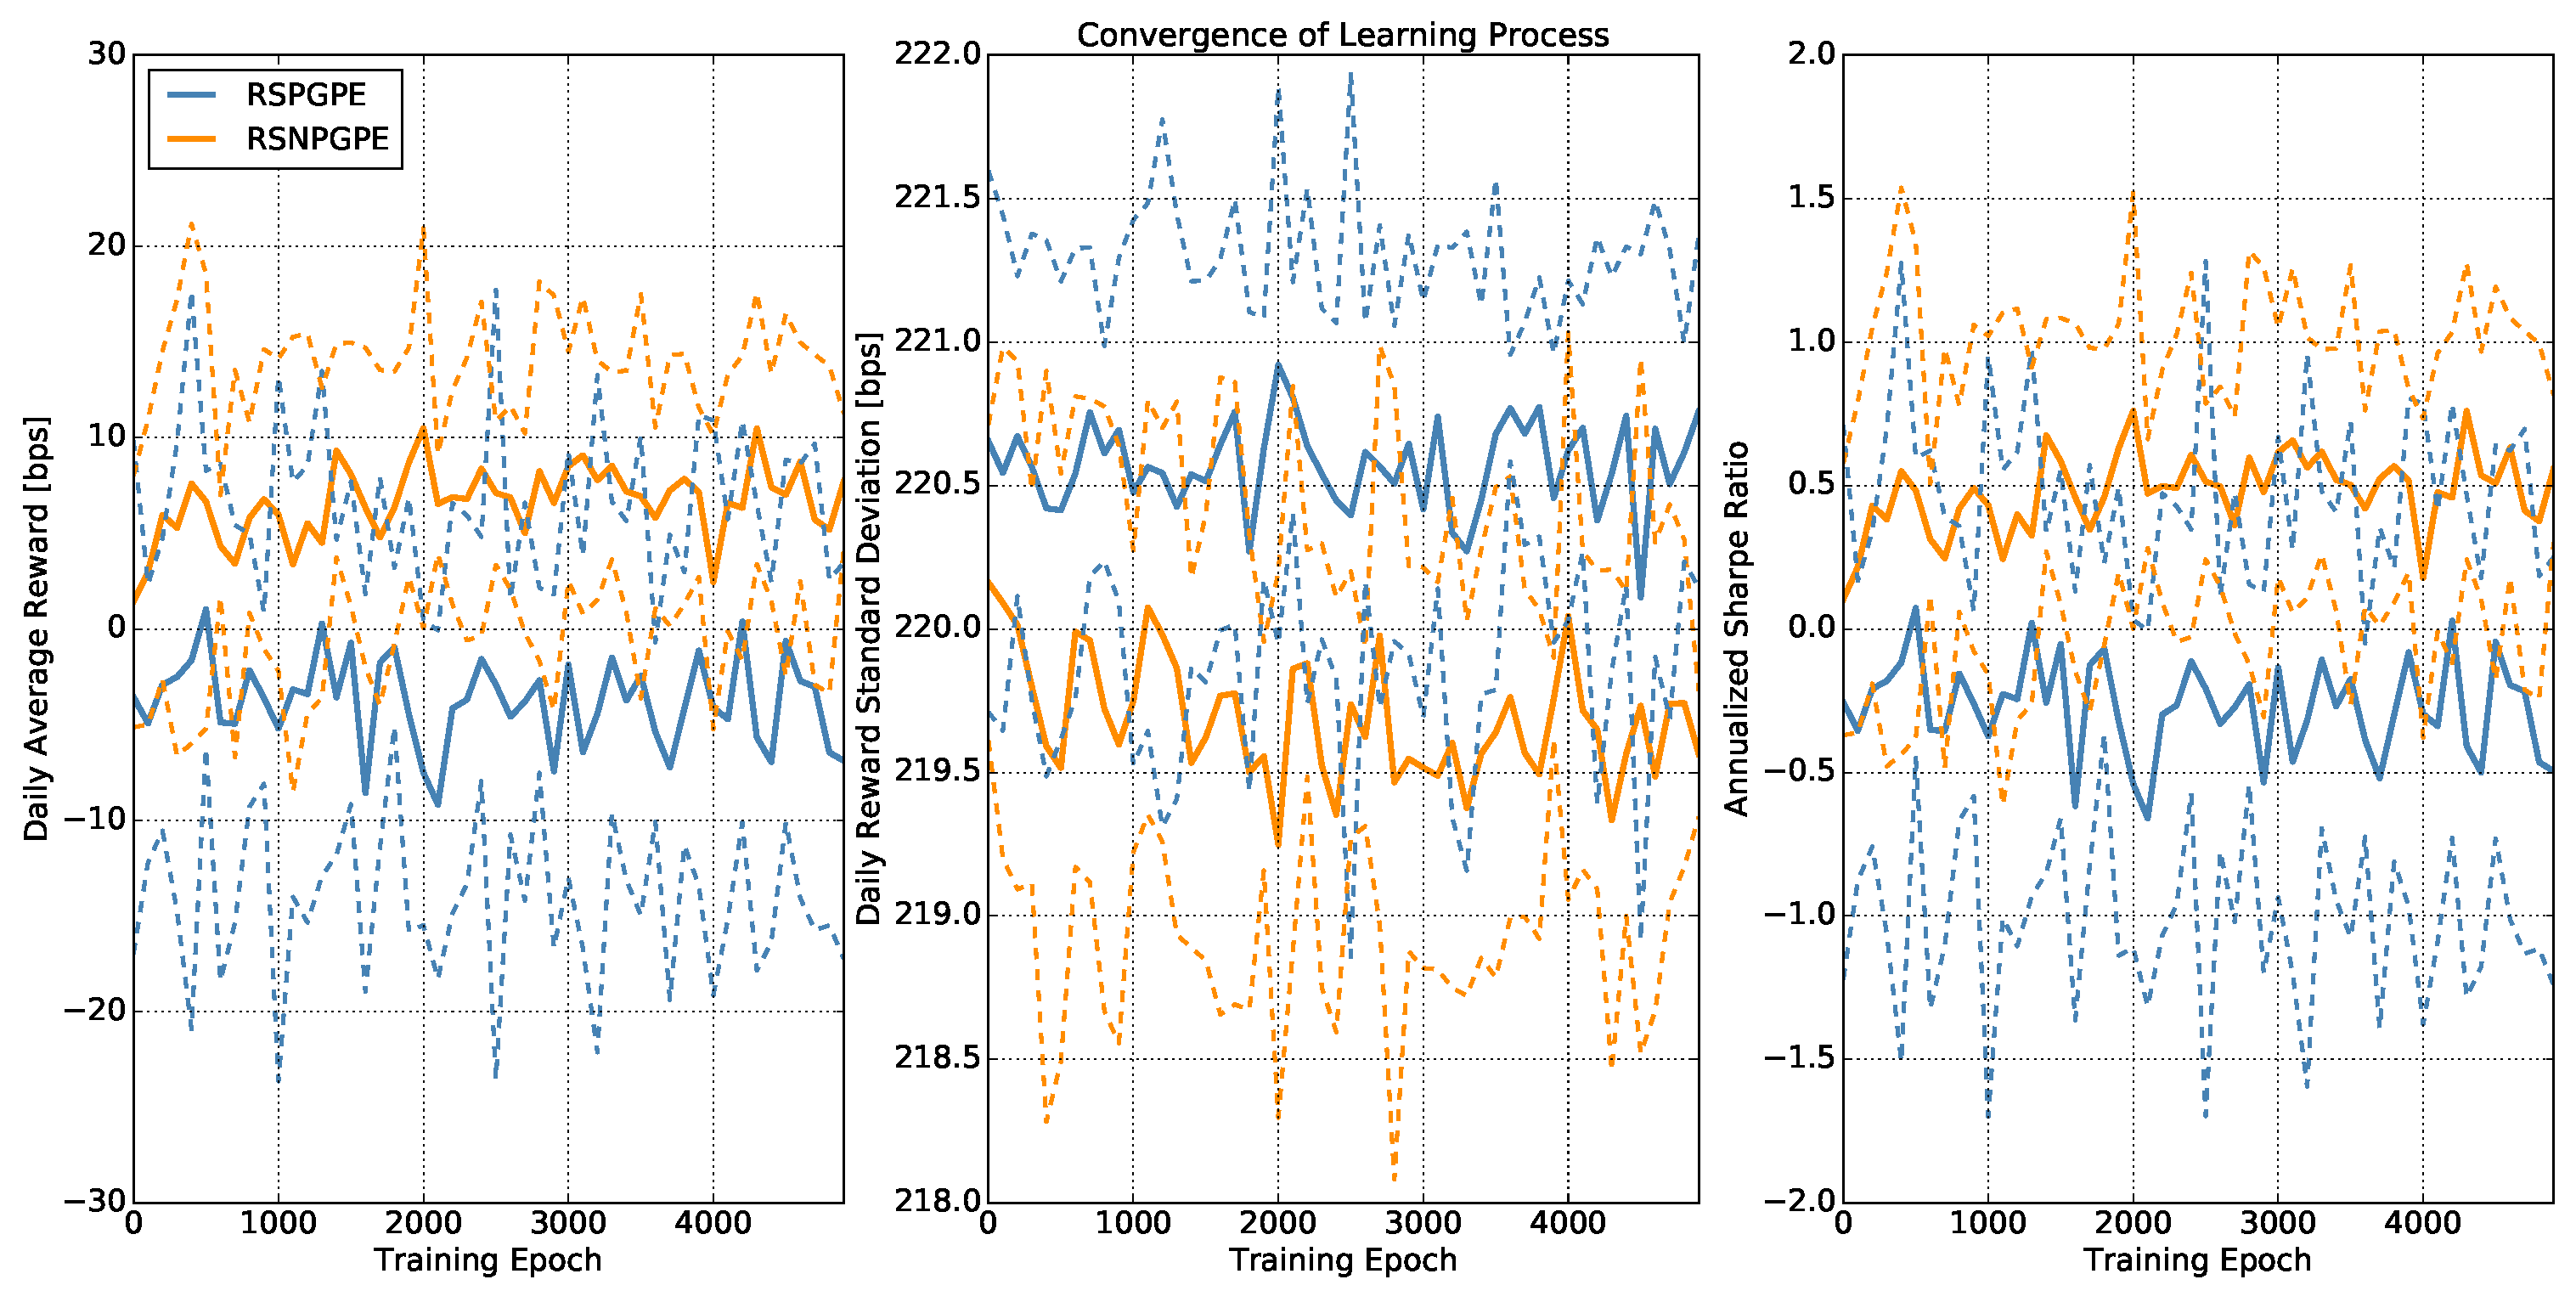
\includegraphics[height=6cm,width=1.0\textwidth]{Images/8_10_single_hist_sensitive_convergence}
	\caption[]{}
	\label{fig:}
\end{figure}

\begin{figure}[t!]
	\centering
	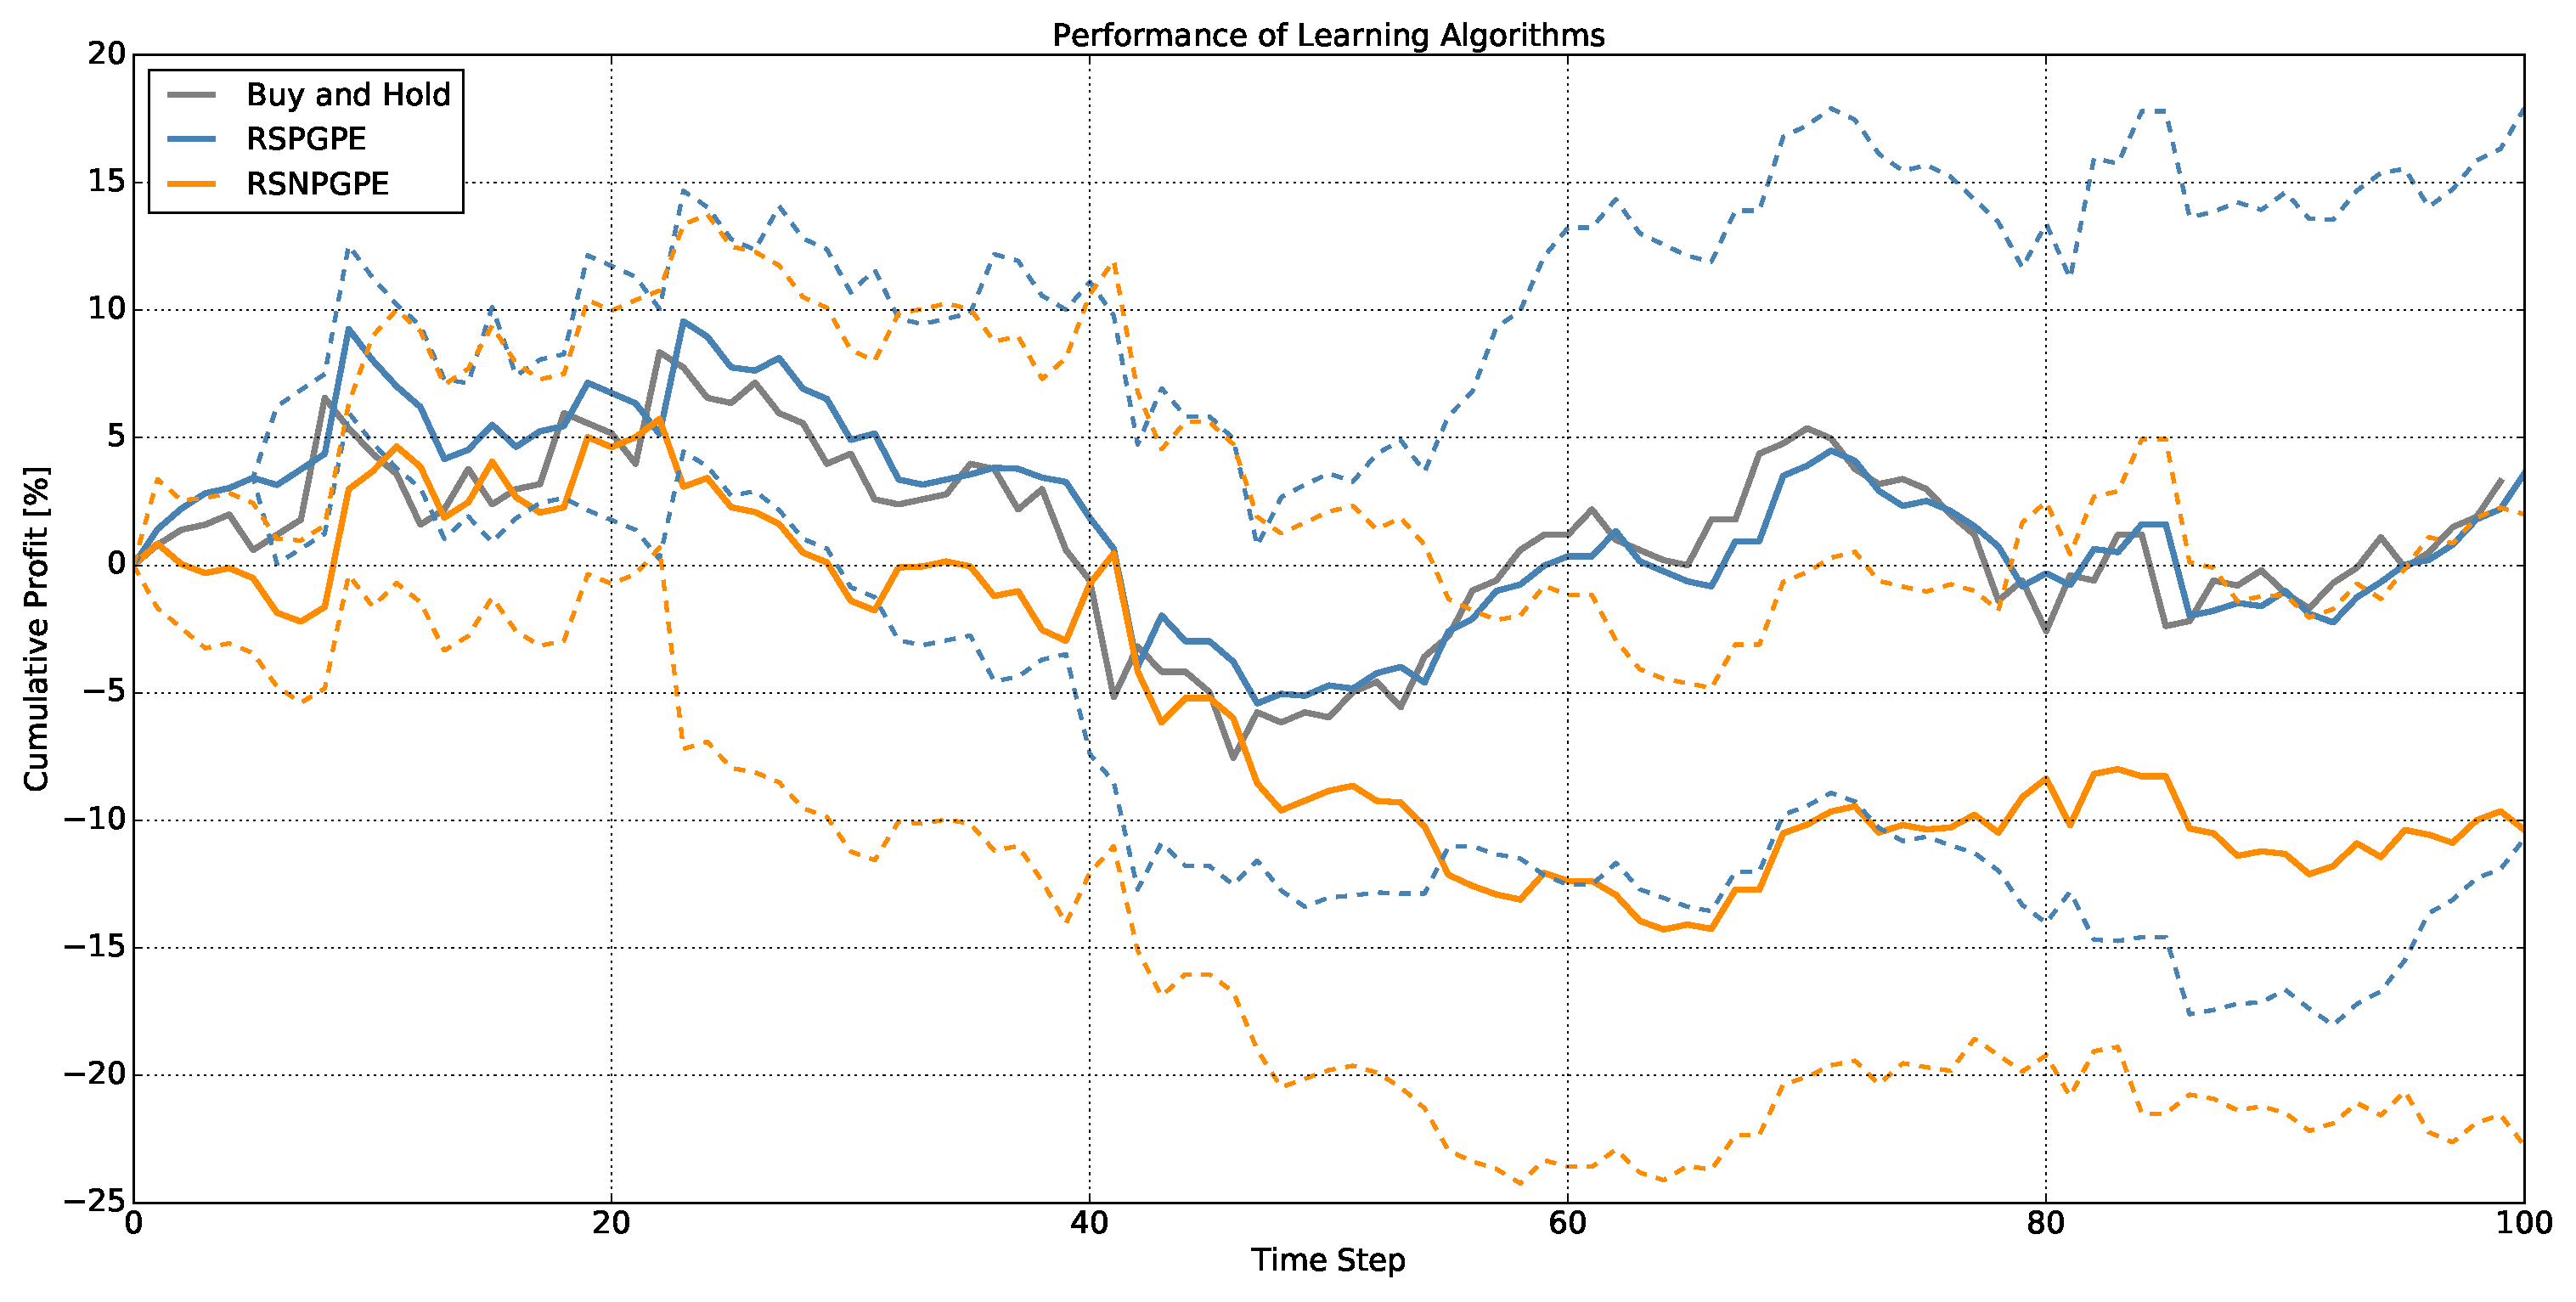
\includegraphics[height=6cm,width=1.0\textwidth]{Images/8_11_single_hist_sensitive_performance}
	\caption[]{}
	\label{fig:}
\end{figure}

\section{Multiple Synthetic Risky Assets}
In this section we present an application of the learning algorithms considered above to a multi-asset allocation problem. Given the difficulties of learning a profitable strategy for historical data, we consider once again synthetic price series that can be traded profitably. To define the generative model, we start from a continuous-time formulation and then derive a discrete-time model using standard discretization techniques. In particular, we assume that the market consists of two risky asset $\{S_t^1, S_t^2\}$, whose prices evolve according to the following dynamics
\begin{equation}
	\begin{cases}
		\frac{dS_t^1}{S_t^1} &= \sigma_1 dW_t^1\\ 
		\frac{dS_t^2}{S_t^2} &= \frac{1}{2} \sigma_\chi^2 dt + \sigma_2 dW_t^2 + d\chi_t\\
		d\chi_t &= -\lambda \chi_t dt + \sigma_\chi dW_t^\chi\\
	\end{cases}
\end{equation}
where $\{W_t^1, W_t^2, W_t^\chi\}$ are standard Brownian motions such that $\E {dW_t^1 dW_t^2} = \rho dt$, with $-1 \leq \rho \leq 1$, $W_t^\chi \independent (W_t^1, W_t^2)$, 
$\sigma_1$, $\sigma_2$, $\sigma_\chi$, $\lambda >0$ and $\chi_0 = 0$. The Ornstein-Uhlenbeck process $\chi_t$ represents a mean-reverting spread between the two risky assets. Let $\widetilde{S}_t^i = \log S_t^i$, $i \in \{1,2\}$ denote the log-price. A simple application of Itô's lemma yields 
\begin{equation}
	\label{eq:sde}
	\begin{cases}
		d\widetilde{S}_t^1 &= -\frac{1}{2} \sigma_1^2 dt + \sigma_1 dW_t^1\\ 
		d\widetilde{S}_t^2 &= -\frac{1}{2} \sigma_2^2 dt + \sigma_2 dW_t^2 + d\chi_t\\
		d(e^{\lambda t} \chi_t) &= \sigma_\chi e^{\lambda t} dW_t^\chi\\
	\end{cases}
\end{equation}
Integrating between $0$ and $t$ and rearranging the various terms, we obtain
\begin{equation}
	\label{eq:sol_sde}
	\begin{cases}
		S_t^1 &= S_0^1 e^{-\frac{1}{2} \sigma_1^2 t + \sigma_1 W_t^1}\\ 
		S_t^2 &= S_0^2 e^{-\frac{1}{2} \sigma_2^2 t + \sigma_2 W_t^2 + \chi_t}\\
		\chi_t &= \sigma_\chi \int_0^t e^{-\lambda (t-u)} dW_u^\chi\\
	\end{cases}
\end{equation}
We notice that the spread is a Gaussian process and $\forall t > 0$
\begin{equation} 
	\chi_t \sim \calN\left(0, \frac{\sigma_\chi^2}{2\lambda}\left(1-e^{-2\lambda t}\right) \right)
\end{equation}
To better understand the role of the spread, let us remind that $W_t^2$ can be decomposed in the following way 
\begin{equation}
	W_t^2 = \rho W_t^1 + \sqrt{1-\rho^2} W_t^{\independent}
\end{equation}
where $W_t^{\independent} \independent W_t^1$ is a standard Brownian motion. Thus, we have 
\begin{equation}
	\frac{S_t^2}{S_t^1} = \frac{S_0^2}{S_0^1} e^{-\frac{1}{2}(\sigma_2^2 - \sigma_1^2) t + (\rho \sigma_2 - \sigma_1) W_t^1 + \sigma_2 \sqrt{1-\rho^2} W_t^{\independent}} e^{\chi_t} 
\end{equation} 
Taking the expected value, we obtain 
\begin{equation}
	\E{\frac{S_t^2}{S_t^1}} = \frac{S_0^2}{S_0^1} e^{\sigma_1 (\sigma_1 - \rho \sigma_2) t} e^{\frac{\sigma_\chi^2}{4\lambda} (1-e^{-2\lambda t})} 
\end{equation} 
The term coming from the stochastic spread disappears in the long term. In the limit case where $\sigma_1 = \sigma_2$ and $\rho = 1$. Then 
\begin{equation}
	\E{\frac{S_t^2}{S_t^1}} = \frac{S_0^2}{S_0^1} e^{\frac{\sigma_\chi^2}{4\lambda} (1-e^{-2\lambda t})} \underset{t \to \infty}{\to} \frac{S_0^2}{S_0^1}
\end{equation} 
Therefore, the expected value of the ratio between the prices of the two risky assets mean-reverts to the initial ratio. It is easy to understand that this feature can be traded profitably by betting on the convergence of the two assets to their long-term regime.\\
The solutions of the system (\ref{eq:sol_sde}) can be easily used to simulate the risky assets prices, which can then be used as inputs of the asset allocation problem. An alternative approach is to obtain the discrete-time dynamics of the system. Let us consider a uniform time-grid $t_k = k \Delta t$, $k \in \mathbb{N}$, and let us integrate the system (\ref{eq:sde}) between $t_k$ and $t_{k+1}$. After some simple algebraic manipulations, we obtain the following equations 
\begin{equation}
	\label{eq:dt_dynamics}
	\begin{cases}
		\widetilde{S}_{k+1}^1 &= \widetilde{S}_{k}^1 -\frac{1}{2} \sigma_1^2 \Delta t + \sigma_1 \sqrt{t} \epsilon_k^1\\ 
		\widetilde{S}_{k+1}^2 &= \widetilde{S}_{k}^2 -\frac{1}{2} \sigma_2^2 \Delta t + \sigma_2 \sqrt{t} \epsilon_k^2 + \chi_{k+1} - \chi_k\\
		\chi_{k+1} &= e^{-\lambda \Delta t} \chi_k + \sigma_\chi \sqrt{\frac{1-e^{-2\lambda \Delta t}}{2\lambda}} \epsilon_k^\chi
	\end{cases}
\end{equation}
where the noises are a Gaussain white noise with the following structure
\begin{equation}
	\begin{bmatrix}
	  	\epsilon_k^1\\
	  	\epsilon_k^2\\
	  	\epsilon_k^\chi\\	  
	\end{bmatrix} \sim \calN\left( 
	\begin{bmatrix}
		  	0\\
		  	0\\
		  	0\\	  
	\end{bmatrix}, 
	\begin{bmatrix}
		  	1, \rho, 0\\
		  	\rho, 1, 0\\
		  	0, 0, 1\\	  
	\end{bmatrix}	
	\right)
\end{equation}
We expect to be possible to trade the two risky assets profitably using an approach similar to the well-known pairs trading technique for cointegrated assets. Intuitively, because of the mean-reversion of the stochastic spread, we should be able to generate a profit by betting on the convergence of the prices of the two assets when they are far apart by selling the more expensive asset and buying the cheaper one. For these considerations, we expect the RL algorithms discussed in the previous chapters to be able to spot this pattern and exploit it to generate a profit. 

\begin{figure}[t!]
	\centering
	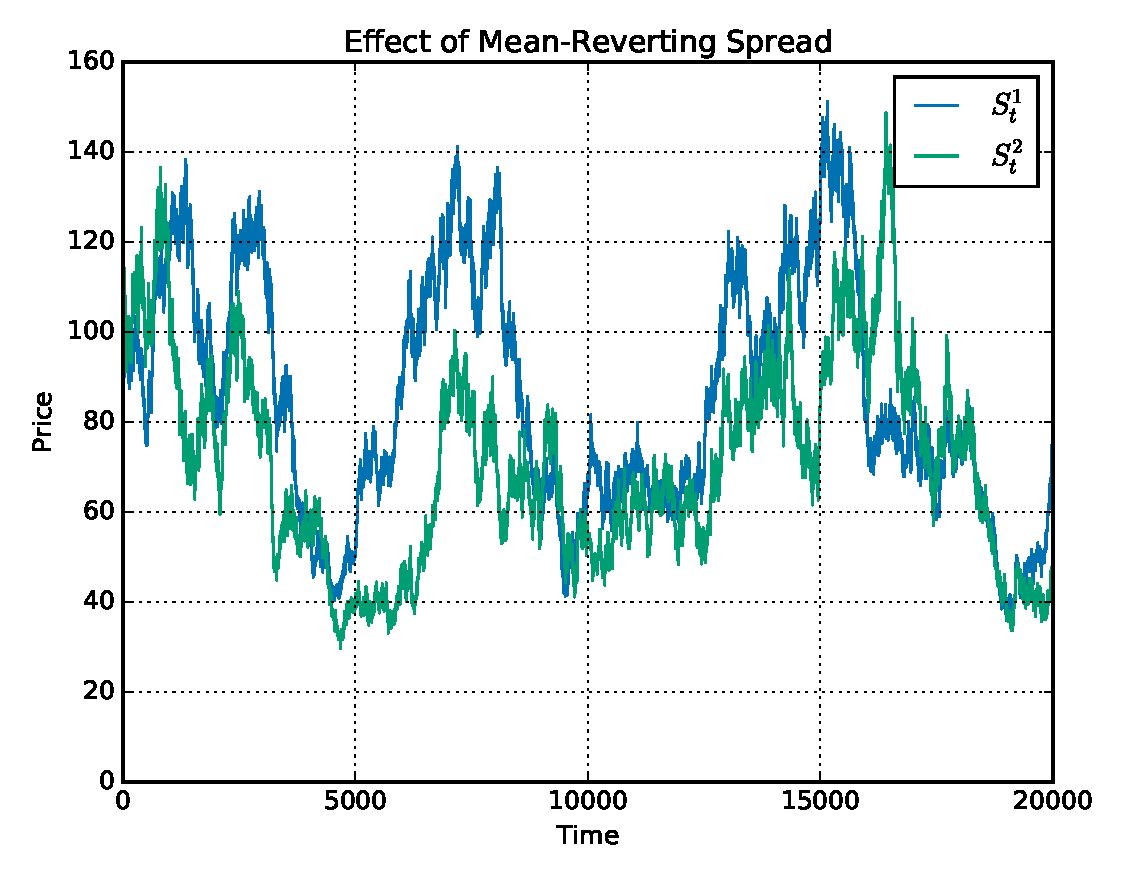
\includegraphics[width=0.8\textwidth]{Images/8_cointegrated_series}
	\caption[Sample paths for the risky assets with a mean-reverting spread.]{Sample paths for the risky assets with a mean-reverting spread.}
	\label{fig:cointegrated_series}
\end{figure}

\subsection{Specifications of the Learning Algorithms}
The parametric policies used in Section \ref{sec:synthetic_risky_asset} can be directly used in this setting to select the weight of one of the assets. Given the poor results obtained with ARAC, we only focus on the PGPE and NPGPE algorithms. The weight on the first asset is selected using The following controller 
\begin{equation*}
	a^1 = F_\theta(s) = \sign(\theta \cdot s)
\end{equation*}
where in PGPE the parameters are sampled from a multi-variate Gaussian distribution
\begin{equation*}
	\theta \sim \calN(\mu, \diag(\sigma))
\end{equation*}  
while in NPGPE the controller parameters are sampled from a Gaussian distribution parameterized by its mean and Cholesky factor
\begin{equation*}
	\theta \sim \calN(\mu, C^T C)
\end{equation*}  
The long-short strategy is completed by selecting $a^2 = - a^1$. In this case we notice that $a^1 + a^2 = 0$, which means that the long position on one asset is entirely financed by the short position on the other asset. Clearly, this assumption is simplistic as it neglects all the practical constraints on short-selling. Given that we will always be short on one of the two assets, we will also neglect short-selling fees, i.e. $\delta_s = 0$. 

